\documentclass[11pt,letterpaper]{article}
\usepackage[T1]{fontenc}
\usepackage[utf8]{inputenc}
\usepackage{amsmath,amsthm}
\usepackage{newtxtext,newtxmath}
\usepackage[margin=0.88in,headheight=15pt,headsep=20pt,footskip=26pt]{geometry}
\usepackage{microtype,mathtools,bm}
\usepackage{booktabs,tabularx,longtable,array,multirow}
\usepackage{graphicx,xcolor,tikz,pgfplots}
\usetikzlibrary{arrows.meta,positioning,calc,fit,backgrounds,shapes.geometric,decorations.pathreplacing}
\pgfplotsset{compat=1.18}
\usepackage{caption,subcaption,float,placeins}
\usepackage{enumitem,listings,fancyhdr,titlesec}
\usepackage[most]{tcolorbox}
\usepackage[numbers,sort&compress]{natbib}
\usepackage{xurl}
\usepackage[colorlinks=true,linkcolor=ink,citecolor=teal,urlcolor=teal,bookmarksnumbered=true]{hyperref}
\definecolor{ink}{HTML}{183247}
\definecolor{teal}{HTML}{126C70}
\definecolor{muted}{HTML}{607381}
\definecolor{paperblue}{HTML}{EEF4F7}
\definecolor{papergreen}{HTML}{EDF6F3}
\definecolor{ochre}{HTML}{99621D}
\definecolor{paperamber}{HTML}{FCF5E8}
\hypersetup{pdftitle={The Work a Verifier Needs},pdfauthor={Samuel Mausberg},pdfsubject={WIP systems research: shared-head certificates and speculative execution}}
\pagestyle{fancy}\fancyhf{}
\fancyhead[L]{\small\textsc{The Work a Verifier Needs}}
\fancyhead[R]{\small\textcolor{muted}{Research draft · 30 September 2026}}
\fancyfoot[L]{\footnotesize\textcolor{muted}{Samuel Mausberg}}
\fancyfoot[R]{\small\thepage}
\renewcommand{\headrulewidth}{0.3pt}
\titleformat{\section}{\Large\bfseries\color{ink}}{\thesection}{0.6em}{}
\titleformat{\subsection}{\large\bfseries\color{ink}}{\thesubsection}{0.6em}{}
\titleformat{\subsubsection}{\normalsize\bfseries}{\thesubsubsection}{0.6em}{}
\titlespacing*{\section}{0pt}{2.0ex plus 1ex minus .2ex}{1.1ex}
\titlespacing*{\subsection}{0pt}{1.7ex plus .5ex minus .2ex}{.7ex}
\setlength{\parindent}{1.1em}\setlength{\parskip}{0.2em}
\setlength{\emergencystretch}{2.2em}
\setlist{nosep,leftmargin=1.6em,topsep=0.5em}
\captionsetup{font=small,labelfont={bf,color=ink},skip=7pt}
\renewcommand{\arraystretch}{1.16}
\newcolumntype{P}[1]{>{\raggedright\arraybackslash}p{#1}}
\newcolumntype{Y}{>{\raggedright\arraybackslash}X}
\newcommand{\E}{\mathbb E}\newcommand{\R}{\mathbb R}\newcommand{\ind}{\mathbf 1}
\newcommand{\argmax}{\operatorname*{arg\,max}}
\newcommand{\lse}{\operatorname{LSE}}
\newcommand{\softmax}{\operatorname{softmax}}
\newcommand{\clip}{\operatorname{clip}}
\newcommand{\norm}[1]{\left\lVert #1\right\rVert}
\newcommand{\code}[1]{\texttt{\small #1}}
\newcommand{\sourcepin}{\texttt{bd66ce343e4f}}
\newtheorem{theorem}{Theorem}[section]
\newtheorem{proposition}[theorem]{Proposition}
\newtheorem{lemma}[theorem]{Lemma}
\newtheorem{corollary}[theorem]{Corollary}
\theoremstyle{definition}\newtheorem{definition}[theorem]{Definition}
\theoremstyle{remark}\newtheorem{remark}[theorem]{Remark}
\newtcolorbox{researchbox}[1][]{enhanced,breakable,colback=paperblue,colframe=ink!30,boxrule=.4pt,arc=1pt,left=9pt,right=9pt,top=7pt,bottom=7pt,#1}
\lstset{basicstyle=\ttfamily\footnotesize,breaklines=true,columns=fullflexible,keepspaces=true,frame=single,rulecolor=\color{ink!20},backgroundcolor=\color{paperblue},showstringspaces=false,aboveskip=9pt,belowskip=9pt}
\tikzset{box/.style={draw=ink!45,fill=paperblue,rounded corners=2pt,align=center,font=\small,inner sep=7pt},good/.style={box,fill=papergreen,draw=teal!60},warn/.style={box,fill=paperamber,draw=ochre!55},flow/.style={-{Stealth[length=2.1mm]},thick,draw=ink},dashedflow/.style={flow,dashed},label/.style={font=\footnotesize,text=muted,align=center}}

\setcounter{tocdepth}{1}
\begin{document}
\begin{titlepage}
\vspace*{0.15in}
\noindent{\small\sffamily\color{teal}SYSTEMS RESEARCH\quad /\quad WORK IN PROGRESS\quad /\quad REVISION 3}\par
\vspace{0.40in}
\noindent{\fontsize{34}{39}\selectfont\bfseries\color{ink}The Work a\par\noindent Verifier Needs\par}
\vspace{0.25in}
\noindent{\Large Shared-head certificates, demand-driven projection,\par\noindent and state-aware speculative execution}\par
\vspace{0.32in}
\noindent{\large Samuel Mausberg}\par
\noindent{\color{muted}30 September 2026}\par
\vspace{0.30in}
\begin{abstract}
\noindent A speculative decoder usually asks its target model for much more information than acceptance requires. A greedy verifier needs a winner; a sampled verifier often needs only the truth of one inequality. Yet both commonly receive a complete vocabulary projection. We investigate whether a drafter's already-paid projection through a shared output head can become a certificate for these later decisions. Tile summaries are transported from draft to target hidden states with deterministic bounds. Verification refines only the unresolved tiles and treats exact residual and bonus sampling as separate completion problems, including a bounded race for sparse-support proposals.

The proposed system connects this mechanism to a demand-aware compiler, alternative executions of the DFlash2 selector, transactional hybrid-model state, and scheduling that accounts for graph tiers and shared weight traffic. We derive the certificate rules and their limits, including a counterexample in which candidate-dependent verification depth biases an otherwise standard sampler. Exact-rational CPU references exercise transport, acceptance, replay and scheduling invariants. A synthetic drift experiment shows why cheaper rejection decisions can be a misleading success: completing the residual distribution can consume nearly the entire head again.

This is a research design with executable mathematical evidence, not a completed performance paper. The central empirical question is whether useful certificates survive real hidden-state geometry, finite-precision evaluation and GPU batching. No GPU speedup, real-model calibration or machine-checked Lean result is claimed.
\end{abstract}
\vfill
\begin{researchbox}
\small\textbf{Research claim to pursue.} A compiler can use the consumer's decision contract, together with reusable evidence from earlier computation, to avoid target work without changing the admitted target semantics. Shared-head speculative verification is the first concrete test of that claim.\par\medskip
\textbf{Evidence in this revision.} Twenty-one mathematical CPU test methods and four local benchmark-client tests passed; the earlier suites were rerun. Native \LaTeX/TikZ figures, source audit, counterexamples and runnable references accompany the manuscript. Lean proof source is included but remains uncompiled. This draft does not reproduce the confidential assignment.
\end{researchbox}
\end{titlepage}
\setcounter{page}{1}
\tableofcontents
\vspace{1em}
\noindent\textbf{Reading paths.} Sections~\ref{sec:question}--\ref{sec:demand} contain the main argument. Sections~\ref{sec:gpu}--\ref{sec:tuning} develop the full systems programme. Sections~\ref{sec:experiments}--\ref{sec:evidence} distinguish experiments to run from evidence already obtained. The appendices specify integration contracts, proof boundaries and the implementation sequence.
\newpage

\section{A question larger than a faster selector}\label{sec:question}
The starting plan correctly refused to equate accepted draft length with performance. It also identified several useful implementation boundaries: the output head, DFlash2's candidate lattice, recurrent-state commit, and graph-aware verification depth. The remaining weakness was that these boundaries appeared mostly as separate opportunities. A stronger paper needs an argument that explains why they belong together.

The argument here is about information. Before choosing a faster implementation of an operation, determine which facts its consumer needs. Then ask whether some of those facts are already implied by earlier work. A tensor that is convenient to produce is not necessarily the right interface. In speculative decoding, the difference is concrete: the target's output head may be asked to produce hundreds of thousands of scores when the next operation needs one comparison.

The particularly useful observation is visible in source rather than inferred from a model name. At the inspected SGLang pin, DFlash's candidate generation projects draft hidden states through the target LM head. The dense path materializes logits and selects candidates; an optional path also computes the partition function.\cite{sgcode} The proposal is to extend this already-required pass so that it produces compact, reusable summaries. When target hidden states arrive, the summaries become bounds on the target projection. The target head is then evaluated as far as the verifier's decision requires, with a complete fallback whenever the bounds are inconclusive.

This does not make the target backbone disappear. Nor does it imply that draft and target hidden states are close in a useful norm. It gives us a specific mechanism whose success or failure can be explained: evidence produced by one head application may replace arithmetic in another application of the same head.

\subsection{The intended contribution}
The central contribution to pursue is a \emph{shared-head certificate execution path}: summary production, bound transport, decision refinement, numerical admission and graph-safe completion. The component inequalities are elementary. The research question is whether their composition can change the amount of work required by an optimized speculative server.

The broader programme remains substantial. It includes a compiler interface for decision consumers, a selector execution portfolio, calibrated prefix-value search, hybrid-state transactions, weight-reuse-aware scheduling and structural autotuning. These are not promised as simultaneous speedups. They are connected hypotheses with explicit composition rules. A useful paper may establish that several of them fail and explain precisely why one survives.

\begin{researchbox}
\textbf{What would make the result strong.} Demonstrate avoided target weight traffic or arithmetic, not just fewer Python calls; preserve a stated target and sampling contract; explain the crossover under concurrency; and attribute the end-to-end effect with ablations against an already optimized speculative baseline. A proof without useful bounds, a sparse mask without reduced traffic, or a faster acceptance test followed by an expensive residual pass does not establish the claim.
\end{researchbox}

\subsection{Model choice is a test of the mechanism}
Qwen3.5-4B remains a useful first experimental target. Its published configuration has hidden width 2,560, vocabulary size 248,320, 24 linear-attention layers and eight full-attention layers, with an MTP component.\cite{qwenconfig,qwencard} A BF16 matrix of that vocabulary and width occupies approximately $1.271$ GB before packing or padding. This is a calculation from the configuration, not a measured allocation. The combination of a large head and hybrid state makes the model interesting without making model size itself the contribution.

The shared-head certificate experiment needs an actually compatible drafter. The inspected public DFlash2 release for Qwen3.8-27B is one verified pairing; this audit does not establish a public Qwen3.5-4B DFlash2 checkpoint.\cite{dflashcard} A compatible small checkpoint supplied with permission would be preferable for the first complete experiment. Native MTP is a separate strong baseline and a possible certificate producer, but its hidden-state alignment, head sharing and runtime path must be checked rather than assumed. A successful mechanism should later transfer to a second architecture and another GPU regime. These transfers enlarge the research claim; they do not justify mixing unlike models in one speedup denominator.

\begin{figure}[t]
\centering
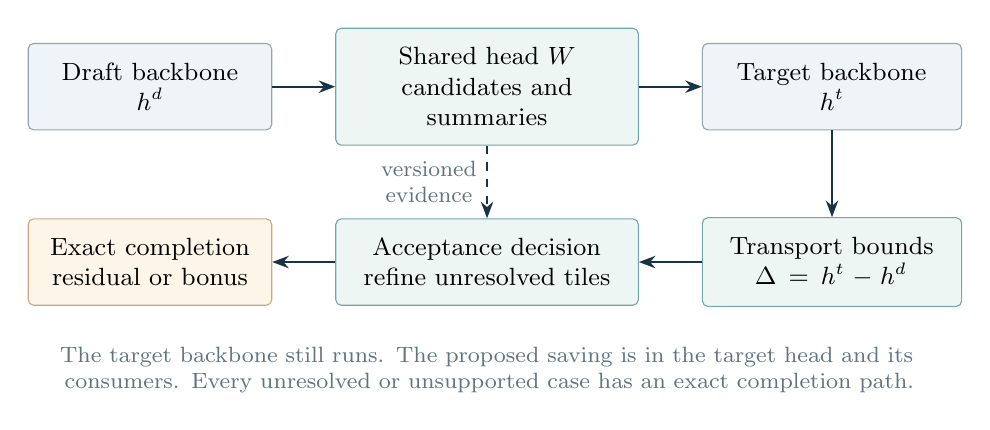
\begin{tikzpicture}[node distance=.8cm]
\node[box,text width=2.6cm] (draft) {Draft backbone\\$h^{d}$};
\node[good,text width=3.35cm,right=of draft] (dh) {Shared head $W$\\candidates and summaries};
\node[box,text width=2.8cm,right=of dh] (target) {Target backbone\\$h^{t}$};
\node[good,text width=2.8cm,below=1.1cm of target] (cert) {Transport bounds\\$\Delta=h^t-h^d$};
\node[good,text width=3.35cm,left=of cert] (dec) {Acceptance decision\\refine unresolved tiles};
\node[warn,text width=2.6cm,left=of dec] (finish) {Exact completion\\residual or bonus};
\draw[flow] (draft)--(dh);\draw[flow] (dh)--(target);
\draw[flow] (target)--(cert);\draw[flow] (cert)--(dec);\draw[flow] (dec)--(finish);
\draw[dashedflow] (dh.south)--node[left,label]{versioned\\evidence}(dec.north);
\node[label,below=.4cm of dec,text width=11.4cm] {The target backbone still runs. The proposed saving is in the target head and its consumers. Every unresolved or unsupported case has an exact completion path.};
\end{tikzpicture}
\caption{The proposed execution path. Summary production is part of the cost of drafting, not free preprocessing. Dashed edges carry reusable evidence; solid edges carry ordinary data or control.}
\label{fig:flow}
\end{figure}

\section{Where prior work already reaches}\label{sec:prior}
A source audit should remove false novelty before experiments make it expensive to abandon. Table~\ref{tab:prior} states the relevant overlap and the narrower question left for this programme. The audit is targeted, not an exhaustive priority search.

\begin{table}[t]
\small\centering
\begin{tabularx}{\linewidth}{@{}P{2.6cm}YY@{}}\toprule
Existing work & Already established or implemented & Question pursued here \\\midrule
DFlash2\cite{dflash,sgcode} & Context-gated candidate correlations and parallel score construction followed by a path walk. & Reuse its head work as evidence; change selector execution without changing its choices.\\
FlashSampling\cite{flashsampling} & Exact categorical sampling fused into the output projection; tile-local Gumbel maxima avoid full logits. & Avoid some projection itself, not merely its materialization.\\
SonicSampler\cite{sonic} & Tile-aware post-logit sampling and verification kernels. & Distinguish exact consumer contracts from restricted-support approximations.\\
SpecVocab, DynaSpec, MicroSpec\cite{specvocab,dynaspec,microspec} & Dynamic or context-conditioned draft-vocabulary restriction. & A bound that preserves the target decision, including explicit mass obligations.\\
ReplaySSM; GDN kernels\cite{replayssm,gdncode} & Input/record replay and accepted-prefix state restoration. & Expose state and lifetime costs to compilation and scheduling.\\
OPT-Tree, D-cut, PR~36136\cite{opttree,dcut,pr36136} & Expected-acceptance structure, adaptive verification depth and cost-aware graph budgeting. & Account for certificate masks and state costs; specify sampled-policy admissibility.\\
Mirage\cite{mirage} & Multi-level search over tensor implementations with its own verification machinery. & Decision-demand and state-effect contracts around the searched subgraphs.\\\bottomrule
\end{tabularx}
\caption{Prior art limits the novelty claim. A source's reported performance is not reproduced by this manuscript.}
\label{tab:prior}
\end{table}

FlashSampling is a material addition to the earlier plan's audit. Its fused projection-plus-sampling kernel is a direct comparator, not a distant citation. It computes complete logits on chip, perturbs them and retains tile maxima.\cite{flashsampling} Our main proposal is different only when transported evidence safely prevents some target rows or tiles from being projected. A fused implementation that still reads the whole head is an integration result and should be described as such.

The vocabulary-restriction literature also matters. SpecVocab, DynaSpec and the versioned MicroSpec manuscript address the expense of draft heads with selected vocabularies.\cite{specvocab,dynaspec,microspec} A changed drafter can remain compatible with an exact target verifier, but its actual proposal law must be used. Our target-side certificate is not the same as assuming that omitted tokens are unimportant. In particular, an omitted logit can contribute to the softmax normalizer even when it cannot win an argmax.

SonicSampler's fixed-size candidate-pool discussion and its treatment of tail mass require care. A top-$K$ operation can be exact as an operation while using that pool for an otherwise unrestricted categorical distribution changes the distribution.\cite{sonic} This is a semantic distinction, not a judgement about whether a quality trade-off is worthwhile. Each experimental arm must identify which law it implements.

LiLiCorr provides a useful warning for the prefix-value branch: its best-path experiment shows that optimizing a different score objective can worsen accepted prefixes. Its characterization of DFlash2 as token-identity-only is not the equation used here; Inco's formulation and the inspected implementation include a hidden-state gate.\cite{lilicorr,dflash,sgcode} We retain the negative decode-rule lesson without importing that simplified model of the selector.

As of this audit, SGLang PR~36136 is open and unmerged. It already proposes confidence-conditioned ragged verification, a profiled cost table and graph-tier alignment. Its reported benchmarks use greedy sampling and show a workload-dependent crossover.\cite{pr36136} The sampled-depth counterexample in Section~\ref{sec:stopping} is \emph{not} evidence that this greedy experiment is incorrect. It identifies an additional obligation before extending such policies to sampling.

\subsection{An explicit novelty boundary}
We do not claim to invent norm bounds, top-$k$ merging, lazy exact sampling, function scans, recurrent replay, graph-aware batching, or proof-guided optimization. A* Sampling is prior art for using bounds to avoid unnecessary work in exact sampling.\cite{astar} The candidate contribution is the particular use of draft-produced shared-head summaries, their verifier-specific refinement protocol, and the compiler/runtime mechanism that makes this useful under actual serving constraints. Priority should be checked again against the exact successful design before submission. Search failure is not evidence of absence.

\section{Semantics before optimization}\label{sec:semantics}
\subsection{Four contracts that must remain separate}
We distinguish mathematical target semantics, a concrete numerical reference, a sampling coupling and a serving observation. Mathematical equivalence over the reals does not imply that two GPU reductions choose the same token. Equality in distribution does not imply identical text under the same seed. Equal token sequences do not imply equal latency or correct cache ownership.

For the first greedy implementation, freeze model weights, adapters, tokenizer, masks, positional settings, intermediate casts and tie-breaking. The verification pass must be checked against ordinary decoding at the committed prefixes. Changes in batching or reduction order can alter close logits even without changing weights.\cite{floatguide,torchnumeric} A deployment may admit a weaker numerical contract, but it must name and evaluate it rather than call it bitwise exact.

For sampled verification, let $p_t$ be the target law at the reached prefix and $q_t$ the \emph{actual} proposal law conditional on the information used to produce that proposal. A softmax buffer from a different selector is not $q_t$. A deterministic proposal is a point mass. A choice among multiple random proposals generally has a different law from each individual proposal.

The standard one-step correction draws $X\sim q$, accepts with probability $\min(1,p_X/q_X)$, and otherwise samples from $(p-q)_+$ normalized. The accepted mass at $i$ is $\min(p_i,q_i)$ and the rejected branch contributes $(p_i-q_i)_+$; their sum is $p_i$.\cite{specdecode} This identity is the boundary to preserve. Our acceptance certificate changes how a comparison is evaluated, not the law used in it.

\subsection{Useful progress and elapsed time}
Let a cycle commit $R$ output tokens and take elapsed time $T>0$. Under a stationary regenerative model with finite expectations, the long-run rate is
\begin{equation}\rho=\frac{\E R}{\E T}.\label{eq:rate}\end{equation}
The result follows from the ratio of accumulated rewards and accumulated times. It is not $\E[R/T]$. Nor is it a queueing-latency model. Away from termination boundaries, an ordinary speculative cycle with $A$ accepted draft tokens often commits $A+1$ tokens; EOS, length limits and streaming conventions require explicit truncation.

A candidate improves this rate exactly when $\E R_1/\E R_0>\E T_1/\E T_0$. This simple condition prevents a recurring mistake: higher acceptance does not compensate for arbitrary overhead. It also prevents the opposite mistake. A lower acceptance rate can be worthwhile when the saved work exceeds the lost progress.

The denominator includes summary generation, draft and target backbones, projection, selection, refinement, residual/bonus completion, state commit, non-overlapped dispatch and policy overhead. A fixed-width target backbone executes admitted positions even if the first proposal will be rejected. Survival probabilities may weight reward; they may weight cost only where work is genuinely conditional. Overlapped kernels require a critical-path measurement rather than an indiscriminate sum of durations.

\subsection{The producer--consumer contract}
The compiler should distinguish at least the following consumers:
\begin{center}\small
\begin{tabularx}{\linewidth}{@{}P{3cm}Y@{}}\toprule
Consumer & Required information \\\midrule
Greedy token & Winning ID under the admitted numerical and tie contract.\\
Exact top-$k$ & Winning IDs and scores; no full partition unless another consumer requires it.\\
Acceptance bit & $\exp(z_X)$ compared with $Uq_XZ$; an interval may suffice.\\
Residual sample & Correct $(p-q)_+$ law, including omitted target and proposal mass.\\
Bonus sample & A sample from the target law, with a specified RNG contract.\\
Arbitrary log-probabilities & Requested logits and the full target partition; often defeats a narrow fast path.\\\bottomrule
\end{tabularx}
\end{center}
A fast path is admitted by these contracts, not by a request merely being labelled ``decode.'' Grammar masks, repetition penalties and temperature transforms are part of the relevant scores. They cannot be applied after winners have already been discarded.

\section{Transporting evidence through a shared head}\label{sec:transport}
\subsection{Tile geometry and already-paid summaries}
Let $W\in\R^{V\times D}$ be the same head used for a draft hidden vector $h^d$ and an aligned target hidden vector $h^t$. Write $\Delta=h^t-h^d$, $z_i^d=\langle w_i,h^d\rangle$ and $z_i^t=\langle w_i,h^t\rangle$. A vocabulary partition $\mathcal C$ is disjoint and covers all admitted tokens. For each tile $c$, choose a centre $\mu_c$ and a radius
\begin{equation}
r_c\geq\max_{i\in c}\norm{w_i-\mu_c}_\infty,\quad
 a_c=\langle\mu_c,\Delta\rangle,\quad
 \epsilon_c=r_c\norm{\Delta}_1.\label{eq:geometry}
\end{equation}
The draft pass emits $M_c^d=\max_{i\in c}z_i^d$ and $Z_c^d=\sum_{i\in c}\exp(z_i^d)$. Stable implementations store a maximum and scaled mass or a log-mass, not an overflowing exponential. The centres and radii are checkpoint metadata; the maxima and masses belong to this request, position and draft hidden vector.

\begin{theorem}[Transported tile certificates]\label{thm:transport}
Under the real-arithmetic shared-head contract, every $i\in c$ satisfies
\begin{equation}
z_i^d+a_c-\epsilon_c\leq z_i^t\leq z_i^d+a_c+\epsilon_c.\label{eq:transport-row}
\end{equation}
Consequently,
\begin{align}
\max_{i\in c}z_i^t&\leq M_c^d+a_c+\epsilon_c=:U_c,\label{eq:maxbound}\\
 e^{a_c-\epsilon_c}Z_c^d&\leq Z_c^t\leq e^{a_c+\epsilon_c}Z_c^d.\label{eq:massbound}
\end{align}
\end{theorem}
\begin{proof}
Subtract $z_i^d+a_c$ from $z_i^t$. The result is $\langle w_i-\mu_c,\Delta\rangle$, whose absolute value is at most $r_c\norm{\Delta}_1$ by H\"older's inequality. Maximization gives~\eqref{eq:maxbound}; monotonicity of the exponential and summation give~\eqref{eq:massbound}.
\end{proof}
The distinction from a static norm screen is important. A static screen bounds a target score from weight geometry and $h^t$ alone. Transport starts from a score or mass already measured at $h^d$ and bounds only the change. It can be substantially tighter when the change is small in a suitable geometry. It can also be useless when that geometry is wrong.

\subsection{A summary that supports both selection and mass}
For a set of labelled logits $S$, define a summary containing its top-$k$ items under descending score then ascending token ID, and the mass of every discarded item. Two summaries merge by selecting the top-$k$ of their retained union and adding the newly discarded mass to the two old tails.

\begin{proposition}[Top-$k$ plus tail is a compositional summary]\label{prop:summary}
For disjoint finite domains, this merge produces the same top-$k$ items and tail mass as summarizing their union. It is associative in exact arithmetic under the common total ordering.
\end{proposition}
\begin{proof}
An item omitted from a local top-$k$ has at least $k$ locally superior items and cannot enter the union's top-$k$. All possible winners are therefore retained. The original tails and newly discarded retained items partition the final tail. Summing their masses gives the correct tail without subtracting nearly equal totals. Every parenthesization represents the same union and thus the same summary.
\end{proof}
This is a sufficient-statistic construction from familiar reductions, not a novel selection theorem. Its value is an interface: one epilogue can serve candidate generation, target bounds and exact completion. It must preserve the reference cast before ranking when that cast affects the order. Selecting winners of partial dot products along $D$ is invalid; cancellation can reverse the ranking after the remaining coordinates are added.

Retaining a small set $R_c$ also tightens mass bounds. Recompute its target logits exactly, and transport only the old tail:
\begin{equation}
\sum_{i\in R_c}e^{z_i^t}+e^{a_c-\epsilon_c}Z^d_{c\setminus R_c}
\leq Z_c^t\leq
\sum_{i\in R_c}e^{z_i^t}+e^{a_c+\epsilon_c}Z^d_{c\setminus R_c}.\label{eq:tail}
\end{equation}
These bounds are no looser than transporting the entire tile with the same radius. Their cost is not zero: $|R_c|$ additional row projections per tile can be worse than waiting for a small number of useful full-tile refinements. Tail mass should be accumulated directly; obtaining it as ``total minus top mass'' can lose the very information being certified.

\subsection{Geometry is the first serious falsification gate}\label{sec:geometry}
A good draft does not imply small $\norm{h^t-h^d}_1$. The head may have directions that do not change its logits, and categorical probabilities ignore a common additive shift. A crude hidden-space norm can charge both heavily. For example, $W=((1,0),(0,0))$ and $\Delta=(0,L)$ leave both logits unchanged for every $L$, yet a tile-wide radius times $\norm\Delta_1$ grows with $L$. This is a defect of the bound, not of the drafter.

We therefore test a hierarchy of bounds. A scalar radius is the cheapest metadata. Coordinate radii give $\epsilon_c=\sum_j r_{cj}|\Delta_j|$. Grouped norms give
\begin{equation}
\epsilon_c=\sum_g r_{cg}\norm{\Delta_g}_2,
\qquad r_{cg}\geq\max_{i\in c}\norm{(w_i-\mu_c)_g}_2.\label{eq:groupbound}
\end{equation}
A low-rank decomposition $w_i=\mu_c+Qu_i+e_i$ allows exact or bounded evaluation of the projected component and a norm bound on $e_i$. Better geometry costs metadata, bound arithmetic and possibly irregular layouts. A learned centre or subspace may improve tightness; learning does not certify the residual radius. That radius must cover the actual stored weights, including the admitted quantization or adapter.

The high-risk extension is to train a drafter for \emph{certificate value} as well as token prediction. A possible objective penalizes measured unresolved mass intervals or head-metric residuals, rather than Euclidean hidden error alone. This must be evaluated against ordinary acceptance-oriented training at equal training cost. A drafter could learn easy-to-certify but unhelpful proposals, or improve certificates while reducing accepted progress. Equation~\eqref{eq:rate} remains the objective.

\subsection{Greedy and top-$k$ admission}
Suppose at least $k$ distinct target rows have been evaluated, and $\tau$ is the score of the $k$th best evaluated item. Skip a tile only when $U_c<\tau$. At least $k$ evaluated items then outrank every skipped item. Strict inequality preserves unresolved ties; score intervals require the tile's upper bound to lie below a valid lower threshold. The same proof applies to a tile's retained tail when its tail maximum was separately summarized.

This establishes exact selection under the specified score contract. It does not establish an exact unrestricted softmax after omitting the tile. A known top-$k$ support can be normalized exactly after its scores are completed; a full-vocabulary top-$p$ threshold has additional mass and ordering obligations. We admit unsupported transform combinations to the ordinary path until those obligations have been implemented.

\section{Evaluate the decision, then refine its demands}\label{sec:demand}
\subsection{An exact acceptance test from incomplete mass}
For one reached proposal $X=x$, write $w_x=e^{z_x^t}$, $Z=\sum_i e^{z_i^t}$ and draw $U\in[0,1)$ with the reference convention. For $q_x>0$, acceptance is equivalent to
\begin{equation}Uq_xZ<w_x.\label{eq:accept}
\end{equation}
The $\min(1,\cdot)$ need not be evaluated explicitly: $U<1$ already handles $p_x/q_x\geq1$.

\begin{theorem}[Acceptance and rejection certificates]\label{thm:guard}
Let $0<Z^-\leq Z\leq Z^+$. Then
\begin{align}
Uq_xZ^+<w_x&\quad\Longrightarrow\quad\text{accept},\\
Uq_xZ^-\geq w_x&\quad\Longrightarrow\quad\text{reject}.
\end{align}
Otherwise the decision is unresolved. Replacing either bound by a tighter valid bound cannot invalidate an already certified decision.
\end{theorem}
\begin{proof}
Multiplication by $Uq_x\geq0$ preserves the ordering of the partition bounds. Each implication follows by transitivity with~\eqref{eq:accept}. Tighter bounds remain on the same side of the true partition, so the same implication continues to hold.
\end{proof}
Transported tile masses provide $Z^-=\sum_c Z_c^-$ and $Z^+=\sum_c Z_c^+$. We compute the candidate's target numerator and test these inequalities before completing any full target tile. An unresolved decision triggers a refinement: replace one or more tile intervals by their exact target mass, update the global bounds and test again. Completing every tile resolves the comparison under the reference convention. This is a finite procedure, not an appeal to a probabilistic confidence estimate.

\begin{proposition}[How much uncertainty remains]\label{prop:unknown}
For fixed $w_x,q_x,Z^-,Z^+$ chosen independently of a uniform $U$ on $[0,1)$, the probability that neither guard decides is
\begin{equation}
P_{?}=\min\!\left(1,\frac{w_x}{q_xZ^-}\right)
      -\min\!\left(1,\frac{w_x}{q_xZ^+}\right).\label{eq:unknown}
\end{equation}
\end{proposition}
\begin{proof}
The unresolved uniforms lie between the acceptance threshold implied by $Z^+$ and the rejection threshold implied by $Z^-$. Intersect that interval with $[0,1)$ and take its length. Endpoints have zero measure under a continuous uniform.
\end{proof}
This expression gives a sharper screening statistic than an average relative error in $Z$. It prices uncertainty where the acceptance threshold lies. It is not automatically the probability of a later adaptive event: after choosing refinements using $U$, one may not treat the resulting bounds as independent of $U$. The guards remain sound pointwise; the probability interpretation needs its stated conditioning.

\subsection{Residual and bonus work cannot be wished away}
A rejected proposal still requires a sample from $(p-q)_+$. Knowing that rejection occurred is not enough to generate that sample. The first implementation therefore completes the target head at the first rejected position and uses the exact reference residual routine. It also retains or reconstructs the actual proposal distribution needed by that routine. When all proposed tokens are accepted, a bonus token still needs a target sample. A strong fused exact categorical sampler, including FlashSampling where compatible, is a comparator and completion candidate.\cite{flashsampling,flashinferapi}

Thus the fast path saves the most when accepted positions can be certified cheaply. It may decide rejection cheaply and save almost nothing after residual completion. That is not an edge case: the synthetic experiment in Section~\ref{sec:evidence} exhibits it directly. A future exact lazy residual sampler is a separate algorithmic branch with its own proof and prior-art comparison; it is not an implicit benefit of the acceptance theorem.

The sparse-support residual race below is a separate, stronger completion candidate. It retains a dense race as its own fallback and comparator rather than silently crediting its possible savings to the acceptance theorem.

\subsection{Exact residual completion with a sparse proposal}
The dense residual fallback is also a baseline for a stronger transformation. Let $Q=\{i:q_i>0\}$ and suppose $|Q|\leq K$. With unnormalized target weights $w_i$ and partition $Z$, the residual distribution can be sampled using weights
\begin{equation}
r_i=(w_i-Zq_i)_+,
\qquad
\frac{r_i}{\sum_j r_j}=
\frac{(p_i-q_i)_+}{\sum_j(p_j-q_j)_+}.\label{eq:residualweights}
\end{equation}
The common factor $1/Z$ cancels. Crucially, $r_i=w_i$ outside $Q$. Only the proposal-support entries need the partition-dependent correction. This branch is admitted only when the \emph{actual} proposal law has that support; it is not inferred from an unrelated top-$k$ candidate buffer.

Let $G_i$ be independent standard Gumbels, independent of the proposal and acceptance randomness. The dense residual race returns $\argmax_i\{\log r_i+G_i\}$, with zero residual weights excluded. Its law is the normalized residual by the ordinary Gumbel-max identity.\cite{flashsampling,astar} We now have a way to bound this race without knowing every target logit or the exact partition.

During a designated draft-head pass, additionally summarize $z_i^d+G_i$ per tile. Reuse \emph{the same} per-token $G_i$ in the target race. Equation~\eqref{eq:transport-row} immediately transports the perturbed scores outside $Q$. Inside $Q$, compute the target weights and use
\begin{equation}
(w_i-Z^+q_i)_+\leq r_i\leq(w_i-Z^-q_i)_+.\label{eq:residualinterval}
\end{equation}
Multiplying these bounds by $e^{G_i}>0$ bounds the candidate's race priority. A winner is certified when its lower priority exceeds every competing upper priority, with the admitted tie rule. Otherwise refine target tiles, which simultaneously tightens $Z$ and the unresolved outside-support race. Complete evaluation is an exact fallback.

\begin{theorem}[Bounded residual-race equivalence]\label{thm:residualrace}
Assume valid target-weight and partition bounds, the actual proposal law, a nonzero residual, and a fixed priority field $e^{G_i}$. A refinement algorithm that returns only an interval-certified ordered maximizer of $r_i e^{G_i}$, or completes the dense race, returns the same token as that dense race. With independent standard Gumbels, it therefore samples the exact residual law in~\eqref{eq:residualweights}.
\end{theorem}
\begin{proof}
Positive-part monotonicity gives~\eqref{eq:residualinterval}; positivity of the priority field preserves the bounds. Outside $Q$, transport encloses the unchanged target weight multiplied by the same priority. The certified candidate dominates every possible competitor, including the actual one. If no candidate is certified, complete evaluation yields the dense ordered maximizer. The distributional statement follows from Gumbel-max applied to the nonzero residual weights.
\end{proof}
A tile maximum that happens to lie inside $Q$ cannot be used as the \emph{exact} outside-support maximum. To handle a support chosen after the draft pass, retain the top $K+1$ perturbed entries per tile. After excluding at most $K$ support IDs, the best remaining entry is present in that list whenever the tile has a remaining entry. If a better omitted entry existed, its $K+1$ retained predecessors could not all have been excluded. This gives an exclusion-aware summary without retaining the entire vocabulary.

The cost is substantial enough to require its own ablation. A separate Gumbel field adds random-number generation and transcendental work to the draft pass; retaining $K+1$ priorities per tile increases epilogue work and evidence traffic. A smaller list with a fallback when exclusions exhaust it is another legal implementation. Reusing the proposal's randomness without a conditional-law argument is not a free optimization: the target race must remain independent of the mechanism that selected the proposal and the rejection event.

The new exact-rational reference implements transported target races, exclusion-aware summaries and the residual-race refinement. It agrees with a dense priority-race reference on the executed finite cases. The test priorities are arbitrary positive rationals, so these tests establish \emph{pathwise algorithmic equivalence}, not an implementation of continuous Gumbel randomness. GPU RNG, numerical priority bounds and useful performance remain untested.

\subsection{A bonus race can use transported evidence too}
For a target-only sample, the same construction is simpler: summarize the tile maxima of $z_i^d+G_i$, transport them, and certify the maximizer of $z_i^t+G_i$. No partition is required. This is an extension of the fused Gumbel-max comparator, with the additional possibility of skipped target projection. It does not make the underlying Gumbel-max method new.\cite{flashsampling}

A bonus row may have no directly aligned draft prediction. Any designated anchor projected through the same head is mathematically valid, but a more distant anchor may give much looser bounds. Producing a distinct bonus-priority summary during the last draft-head pass is one candidate; whether the extra work is worthwhile must be measured. Logical token position and draw purpose, not compacted batch slot, identify the RNG field.

The appropriate comparison for seeded path equality is dense race versus bounded race with the same priority field. An existing inverse-CDF sampler will generally produce different seeded text even when both have the same target law. Report this as a sampler-backend change with distributional and numerical obligations, not as bitwise agreement with the old sampler.

\subsection{A demand frontier over a fixed speculative protocol}
Consider the target head rows for a fixed block of $L$ proposals. Each row is labelled accepted, rejected or unresolved. The first certified rejection at position $r$ proves that no head row after $r$ can affect this cycle's committed output. Earlier unresolved positions still matter: one of them may be the true first rejection. A prefix of certified accepts can be finalized only until the first unresolved or rejected position.

\begin{proposition}[Safe suppression after a certified rejection]\label{prop:frontier}
If every issued certificate equals the decision of a fixed reference verifier on that row, the first true rejection is no later than the first certified rejection. Suppressing head work strictly after the latter does not change the reference cycle output, provided residual/bonus completion and state commit use the actual first rejection.
\end{proposition}
\begin{proof}
At the certified rejection the reference decision is rejection. An earlier unresolved row may also reject; no later row can be the first rejection. All accepted outputs and the replacement are determined by rows up to the first rejection. The required state prefix is determined by the same position.
\end{proof}
The target backbone has ordinarily already evaluated all admitted positions. This frontier saves projection or downstream work, not those completed transformer layers. An interleaved backbone verifier that genuinely stops later layer work is a much larger execution change and needs separate dependencies, causal-state and numerical analysis.

\begin{figure}[t]
\centering
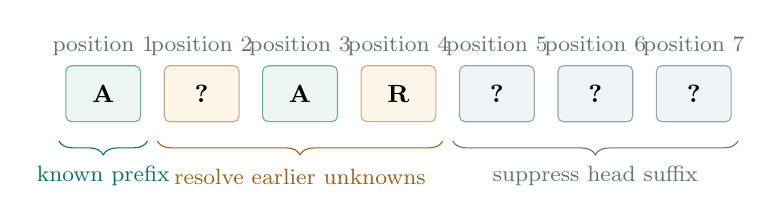
\begin{tikzpicture}[x=1.25cm,y=1cm]
\foreach \i/\txt/\sty in {0/A/good,1/?/warn,2/A/good,3/R/warn,4/?/box,5/?/box,6/?/box}{
  \node[\sty,minimum width=.95cm,minimum height=.7cm] (p\i) at (\i,0) {\textbf{\txt}};
  \node[label] at (\i,.6) {position \the\numexpr\i+1\relax};
}
\draw[decorate,decoration={brace,mirror,amplitude=5pt},draw=teal] (-.45,-.6)--(.45,-.6);
\node[label,text=teal] at (0,-1.05) {known prefix};
\draw[decorate,decoration={brace,mirror,amplitude=5pt},draw=ochre] (.55,-.6)--(3.45,-.6);
\node[label,text=ochre] at (2,-1.05) {resolve earlier unknowns};
\draw[decorate,decoration={brace,mirror,amplitude=5pt},draw=muted] (3.55,-.6)--(6.45,-.6);
\node[label] at (5,-1.05) {suppress head suffix};
\end{tikzpicture}
\caption{A fixed-protocol demand frontier. The rejection at position four makes the suffix irrelevant, but the unknown at position two must still be resolved. Changing evaluation order is different from changing which random proposals the sampling protocol admits.}
\label{fig:frontier}
\end{figure}

\subsection{When adaptive verification changes the sampling law}\label{sec:stopping}
There is an important difference between avoiding work whose result is already determined and deciding which sampled proposals should count. Consider a two-token vocabulary with $p=q=(1/2,1/2)$. Draw a proposal $X$. If $X=0$, discard it and draw a fresh token from $p$. If $X=1$, admit it to the ordinary verifier. Because $p=q$, an admitted proposal is always accepted. The output law is
\begin{equation}
\Pr(Y=0)=\tfrac12\cdot\tfrac12=\tfrac14,
\qquad
\Pr(Y=1)=\tfrac12+\tfrac12\cdot\tfrac12=\tfrac34.\label{eq:bias}
\end{equation}
The verifier's usual acceptance formula was unchanged. The policy was nevertheless biased because admission selected proposals by their realized value. A mandatory first-token progress floor does not fix this construction: apply it to the second position after either first token.

A sufficient safe design chooses a depth before the corresponding proposal randomness is drawn, or makes a stopping decision using the accepted prefix and admissible side information that does not inspect the next proposal draw. The conditional proposal law must still be correct for that information. Confidence scores that are fixed before sampling and token-dependent scores computed after sampling are not interchangeable. More general candidate-dependent policies may be valid with a correctly derived joint law, but the ordinary $p/q$ buffer does not supply that derivation.

Our demand-frontier implementation takes another route: it preserves a fixed reference protocol for every proposal and uniform, and changes only the amount and order of arithmetic used to determine its decisions. Pointwise equality of the protocol output gives a stronger argument than assuming that a scheduler's use of a verifier is sufficient. Greedy decoding has no corresponding proposal-law issue, although its target and state invariants still apply.

\section{Numerical certificates are an implementation obligation}\label{sec:numerics}
Theorems~\ref{thm:transport} and~\ref{thm:guard} are real-arithmetic statements. A production certificate is a statement about a specified implementation. These should not be conflated in either the paper or the code.

\subsection{The reference value must be inside the interval}
Let $\widehat z_i^{\rm ref}$ denote the logit produced by the admitted target implementation, including its casts. A safe bound must enclose this value, not merely the ideal dot product $\langle w_i,h\rangle$. A complete error budget includes the reference reduction, the draft summary's reduction and storage, the centre and radius representation, evaluation of $\Delta$, the bound arithmetic, and any score transform. FMA, reduction order and finite-precision accumulation can change results.\cite{floatguide}

For a textbook sequential floating dot product without exceptional values, a $\gamma_n$-style envelope can bound accumulated rounding in terms of $\sum_j|w_jh_j|$. That formula is not a blanket contract for a tensor-core kernel with different accumulator behaviour. The chosen backend needs an appropriate error model or a compatible reference-evaluation path. A slow conservative bound is acceptable as a correctness reference; whether it remains useful is an experimental question.

The same issue applies to mass. Directed or explicitly inflated bounds must contain the reference exponential and normalization behaviour. An interval enclosing the mathematical softmax of rounded logits need not reproduce every bit of an engine's approximate softmax. The initial artifact therefore distinguishes two specifications: the mathematical law used in the exact CPU references, and the finite reference decisions to be admitted on GPU. Any claim of matching an existing server must discharge the second specification.

With uncertain numerator and denominator, the general guard compares enclosures. If $N^-\leq w_x\leq N^+$ and $D^-\leq Uq_xZ\leq D^+$, then $D^+<N^-$ certifies acceptance and $D^-\geq N^+$ certifies rejection. All remaining cases run the reference path. This phrasing also accommodates rounding in the comparison operands. A uniform stored as a finite bit pattern should be treated according to the reference's actual comparison convention.

\subsection{Stable arithmetic, ties and exceptional cases}
Use maximum-plus-scaled-mass summaries or log-domain inequalities. An all-masked domain has zero mass and cannot be processed by subtracting $-\infty$ from itself. Reject invalid distributions or use the engine's documented fallback. Nonfinite inputs, an invalid radius, an adapter-version mismatch or an unsupported penalty do not produce an optimistic certificate.

A common total order makes top-$k$ proofs precise. It does not prove compatibility with arbitrary library ties; PyTorch explicitly does not promise stable tied indices for \code{topk}.\cite{torchtopk} Preserve the deployed rule where equality is required. Near-tied scores require exact completion or a disclosed numerical contract.

Masks deserve more than a namespace string. If draft and target rows have different grammar states, an unmasked maximum may remain a conservative upper bound, but the old mass is not generally a valid lower bound for the masked target. Prefix-dependent repetition penalties can differ at successive speculative positions. One can derive bounded transform corrections or partition metadata by compatible mask classes; otherwise the request must fall back. A namespace prevents stale evidence from being reused accidentally. It does not make incompatible transformations mathematically equivalent.

\subsection{Progressive precision without changing the target}
A second major research branch uses a cheap head approximation as a certificate producer rather than as the final target. Let $\widetilde z_i$ be a low-precision or low-rank estimate with a proved error envelope $e_i$. A winner is fixed if its lower score exceeds every competing upper score. Acceptance is fixed if every probability consistent with the envelope yields the same comparison. Otherwise refine the relevant rows or run the ordinary target head.

This differs from quantizing the target and accepting quality loss. The reference target remains fixed; approximation changes the cost of proving its decision. The hard part is producing tight, inexpensive envelopes for packed weights and hardware reductions. A branch that cannot provide such envelopes belongs in the approximate-target quality/performance study, not under an exactness label.

\section{Mapping the demand to the GPU}\label{sec:gpu}
\subsection{A kernel family rather than one universal kernel}
The proposed implementation has several shapes. The draft head epilogue produces candidate IDs and tile evidence. A small bound kernel computes centre shifts and residual radii. A target candidate kernel produces numerator or seed scores. A decision kernel identifies unresolved rows and the current rejection frontier. Refinement kernels project selected target tiles, and a completion path handles residual or bonus sampling. These kernels share a stable buffer interface so that fusion and staging can be compared without changing semantics.

Three execution families should be implemented. A conservative two-stage path produces masks then runs compact tile work. A fixed-stage graph path runs a bounded number of guarded refinement rounds before dense completion. A persistent work-queue path may reduce launches, but must be compared against the simpler families rather than presumed superior. Ordinary inter-block spin barriers are not a safe substitute for a legal global synchronization mechanism.

For a head $H W^\top$ with $M$ rows, dense arithmetic is approximately $2MVD$ FLOPs. One ideal weight stream is $b_wVD$ bytes. Avoiding a store and read of materialized logits saves approximately $2b_zMV$ bytes, a ratio $2b_zM/(b_wD)$ to that weight stream. At low $M$, fusion alone may save little head traffic. Transport matters only when it avoids enough projection work to pay for evidence, bound evaluation and reduced GEMM efficiency.

\begin{equation}
T_{\rm evidence}+T_{\rm bounds}+T_{\rm seeds}+T_{\rm refinement}
+T_{\rm completion}<T_{\rm strong\ head\ baseline}.\label{eq:headgate}
\end{equation}
Equation~\eqref{eq:headgate} is a measurement criterion, not a prediction. Repeated tile reads, occupancy loss and graph padding belong in its left side. If a disjoint critical-path component occupies fraction $f$ of total time, eliminating it entirely gives at most $1/(1-f)$ overall speedup under an otherwise unchanged execution. The certificate branch should be rejected early when this ceiling is too small for its overhead.

\subsection{Sparse rows do not imply sparse weight traffic}\label{sec:union}
For microbatch rows $i$, let $A_i$ be the set of retained vocabulary tiles. A tile-major kernel that reuses weights across rows reads the union $\bigcup_i A_i$, not the average of the masks. Under an illustrative model in which each row independently retains a tile with probability $f$, the probability that the batch needs that tile is
\begin{equation}1-(1-f)^B.\label{eq:union}\end{equation}
At $f=1/16$ and $B=32$, this is about $87.3\%$. A reported $93.75\%$ per-row skip fraction can therefore coexist with nearly a full weight stream. This is an analytic example, not a measurement of mask independence in DFlash2.

At the other extreme, running every row independently repeats weight reads and sacrifices tensor-core reuse. The best policy depends on mask correlation, effective $M$, head residency in cache, and the cost of packing work. A useful scheduling objective prices the weighted union of tiles, with an additional term for the number of active row--tile pairs and the resulting execution waves. Similarity grouping can reduce union cost, but must not delay a request indefinitely to find a convenient partner.

\begin{figure}[t]
\centering
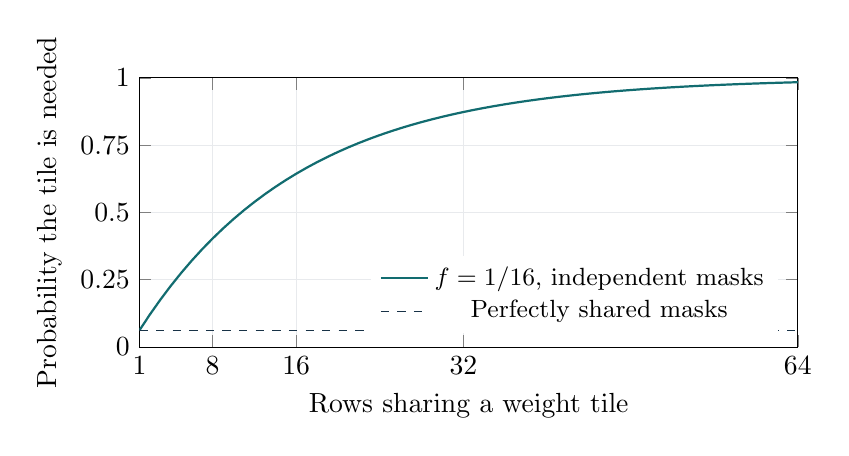
\begin{tikzpicture}
\begin{axis}[width=.82\linewidth,height=5.0cm,xlabel={Rows sharing a weight tile},ylabel={Probability the tile is needed},xmin=1,xmax=64,ymin=0,ymax=1,xtick={1,8,16,32,64},ytick={0,.25,.5,.75,1},grid=major,grid style={draw=ink!10},legend style={at={(.97,.05)},anchor=south east,draw=none,fill=white,font=\small}]
\addplot[thick,teal,domain=1:64,samples=64]{1-(15/16)^x};\addlegendentry{$f=1/16$, independent masks}
\addplot[dashed,ink,domain=1:64,samples=2]{1/16};\addlegendentry{Perfectly shared masks}
\end{axis}
\end{tikzpicture}
\caption{A model of batch-union traffic, not a benchmark. Correlation among certificate masks determines whether per-row sparsity becomes reduced weight traffic. The perfectly shared case assumes all rows retain the same random subset.}
\label{fig:union}
\end{figure}

\subsection{Resource-aware tiling and epilogues}
For a conventional staged GEMM, a first shared-memory filter is
\begin{equation}
S\approx n_s b B_K(B_M+B_N)+S_{\rm epilogue}+S_{\rm barriers}.
\end{equation}
An FP32 accumulator tile requires roughly $4B_MB_N$ bytes distributed across its mapping. These estimates are admission filters, not occupancy predictions. The compiled register count, spills, tensor-memory use where applicable, and active waves must be inspected. A wide vocabulary tile reduces summary traffic but may provide too few workgroups at low $M$. A narrow tile improves parallelism while increasing summaries and merge work.

Compare a strong GEMV/small-GEMM backend with a fused tensor-core kernel rather than forcing every shape through one design. Split-$K$ can increase parallelism but adds a reduction and changes arithmetic order. Epilogue fusion must retain any intermediate rounding that determines candidates or probabilities. The draft summary epilogue can also worsen the draft head enough to erase later savings; its overhead is the first isolated ablation.

Triton, TileLang and CuTe DSL provide different levels of control. We use them as candidate implementation backends, not as evidence that a result is fast. CuTe exposes explicit layout and hardware primitives; TileLang supplies a tile-programming and pipelining interface; Triton supports compact custom kernels and configurable autotuning.\cite{cute,tilelang,tritonautotune} Compiler-generated machine code and resource reports decide whether a mapping is viable.

\subsection{Hardware regimes and graph-safe execution}
Record the actual GPU, compute capability, clocks, memory capacity, driver and compiler. Hopper's TMA and warp-group execution constraints are not interchangeable with all Blackwell devices. In particular, the data-centre and consumer Blackwell targets expose different supported paths; branding is not an instruction-set contract.\cite{hopper,blackwell} A GH200 run that spills weights into CPU memory is a different experiment from a single-GPU-resident run.

The graph-safe design uses fixed maximum buffers, device-resident valid-row and tile masks, stable addresses, and bounded stage counts. A guarded stage that executes no useful work still costs a launch and may incur bookkeeping. Dynamic host reads of a mask can reintroduce synchronization. Full and piecewise graph policies must be measured in their supported serving configurations.\cite{vllmgraphs} A captured candidate cannot be compared only against an eager baseline.

Use Nsight Systems to establish the wall-clock critical path and overlap. Use Nsight Compute on selected kernels to inspect traffic, utilization and stalls; replay and cache-control settings change what a profiling run measures.\cite{nsight} Final throughput measurements should not run under a multipass profiler. Repeating one tensor in a microbenchmark can create a much warmer cache than production. Both realistic and deliberately warm conditions should be labelled.

\section{Compiling the DFlash2 selector in three ways}\label{sec:selector}
The selector remains a research lane because its structure admits different amounts of work and parallelism. At the inspected implementation, adjacent candidate scores have the form
\begin{equation}
S_t(a,b)=U_t(b)+\sum_{r=1}^{d_s}A(a)_r\,H(h_t)_r\,B(b)_r.\label{eq:selector}
\end{equation}
The gate depends on the draft hidden state; it is not an identity-only transition table.\cite{dflash,sgcode} All-pairs construction followed by a walk, realized-row evaluation, and finite-map composition are distinct implementations of the same greedy decision rule.

\subsection{Realized rows: less work, longer dependence}
A greedy walk uses only $S_t(x_{t-1},\cdot)$ at each position. Computing that row when needed reduces score contraction work from $O(BLK^2d_s)$ to $O(BLKd_s)$. With identical inputs, score arithmetic and tie-breaking, induction on $t$ proves the selected path is unchanged. Sampling has the analogous pathwise result only with the same realized proposal rows, row normalization and uniforms.

The lost parallelism can dominate. A full lattice exposes many contractions; a single request's lazy walk exposes a sequence of small dependent contractions. Candidate vectors, hidden gates and gathered tables may not fit in registers without spilling. Evaluate upstream compiled lattice-plus-walk, a fused realized-row kernel, and a partially staged version at actual graph-padded shapes. Do not infer a $K$-fold kernel speedup from a $K$-fold contraction reduction.

\subsection{Finite maps: preserve parallel scoring, compress its consumer}
For greedy selection define $f_t(a)=\argmax_b S_t(a,b)$. Once the row winners are known, the path is
\begin{equation}x_t=(f_t\circ f_{t-1}\circ\cdots\circ f_1)(x_0).
\end{equation}
Each map has $K$ entries rather than $K^2$ scores. A score epilogue can write the winner for every predecessor directly. Chronological composition of maps is associative, so their prefix compositions can be evaluated with a parallel scan.

\begin{proposition}[Finite-map execution]\label{prop:maps}
Given the same row winners, serial map walking and prefix composition produce the same path. A work-efficient scan of length $L$ over $K$-entry maps uses $O(LK)$ map work and $O(\log L)$ composition stages, excluding the score producer.
\end{proposition}
\begin{proof}
The $t$th prefix composition applies exactly the first $t$ transitions to the anchor. Associativity follows from function composition. A work-efficient tree scan uses $O(L)$ compositions, each requiring $O(K)$ indexed evaluations, with logarithmic tree depth.
\end{proof}
The included CPU scan is the simpler Hillis--Steele reference: $O(LK\log L)$ work. It verifies the path equivalence, not an implementation of the work-efficient bound. For short blocks, a serial walk through a small map table may still be fastest. The GPU experiment should compare all three, including the cost of producing maps. Function scanning is a standard parallel technique; the research result would be its profitable placement inside this selector's execution.

A further compression is possible when several predecessors provably have the same successor. For a reference predecessor $a_0$, let $b^*=f_t(a_0)$. If its margin over every $b\neq b^*$ exceeds a bound on
\begin{equation}
\left|\left\langle(A(a)-A(a_0))\odot H(h_t),\,B(b^*)-B(b)\right\rangle\right|,
\end{equation}
then $f_t(a)=b^*$. A norm bound proves this implication by comparing the two score differences. Testing whether enough rows share certified successors is a cheap replay experiment. Computing the bound may cost more than scoring the row, so it is a candidate, not an assumed saving.

\begin{figure}[t]
\centering
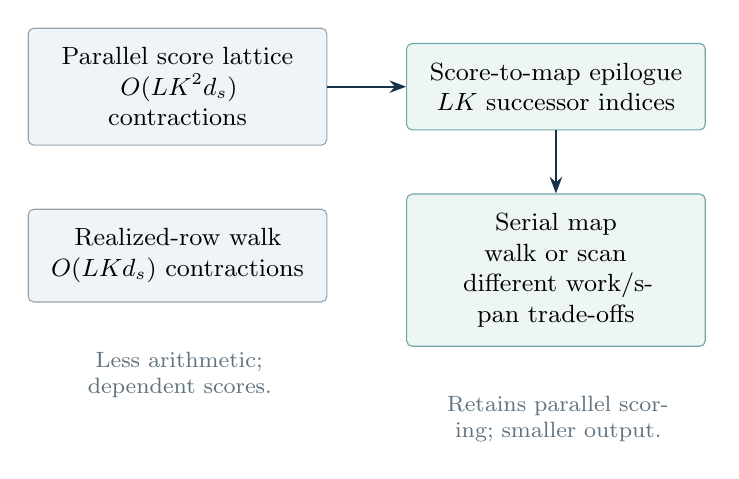
\begin{tikzpicture}[node distance=.5cm]
\node[box,text width=3.3cm] (lattice) {Parallel score lattice\\$O(LK^2d_s)$ contractions};
\node[good,text width=3.3cm,right=1cm of lattice] (maps) {Score-to-map epilogue\\$LK$ successor indices};
\node[box,text width=3.3cm,below=.8cm of lattice] (lazy) {Realized-row walk\\$O(LKd_s)$ contractions};
\node[good,text width=3.3cm,below=.8cm of maps] (scan) {Serial map walk or scan\\different work/span trade-offs};
\draw[flow] (lattice)--(maps);\draw[flow] (maps)--(scan);
\node[label,below=.5cm of lazy,text width=3.5cm] {Less arithmetic; dependent scores.};
\node[label,below=.5cm of scan,text width=3.7cm] {Retains parallel scoring; smaller output.};
\end{tikzpicture}
\caption{Selector alternatives. Lazy scoring and full lookahead do not compose by multiplying their notional savings. Map compression is exact only after row-winner equivalence, including numerical ties, has been established.}
\end{figure}

\subsection{Prefix value is a separate statistical experiment}
The earlier prefix-value dynamic programme remains in scope. On a fixed lattice, suppose $r_t(a,b)$ is a substochastic surrogate for the probability of matching the next target token conditional on a matched prefix and predecessor $a$. For a path $x$,
\begin{equation}
J_r(x)=\sum_{j=1}^{L}\prod_{t=1}^{j}r_t(x_{t-1},x_t),\qquad
V_t(a)=\max_b r_t(a,b)\bigl(1+V_{t+1}(b)\bigr),\quad V_{L+1}=0.
\end{equation}
The recurrence is optimal for the stated Markov surrogate by backward induction. It does not prove that the surrogate describes the target. If edge errors are uniformly bounded by $\epsilon_t$, telescoping prefix products gives $|J_r-J_{\hat r}|\leq\delta=\sum_t(L-t+1)\epsilon_t$, and optimizer regret at most $2\delta$. Average calibration error is not a uniform bound.

Collect candidate lattices at fixed target-greedy anchors independent of the tested selector, and record the true continuation. Compare upstream greedy, raw-score best path, uncalibrated prefix utility, calibrated prefix utility and an oracle coverage ceiling. Split by prompt before fitting. Training only on true-prefix rows does not validate arbitrary off-path histories. A small coverage predictor can account for target tokens outside the candidate pool, but richer context models must pay their inference cost and survive held-out evaluation.

The head certificate and prefix-value objectives may compete. A selector that improves acceptance could move target and draft head geometry into a less certifiable regime; a certificate-friendly drafter could reduce acceptance. The correct experiment measures their joint progress and time. Realized-row greedy does not supply all continuation values required by full lookahead, so those two paths are alternatives unless a new shared computation is explicitly derived.

\section{Hybrid state as a transaction}\label{sec:state}
Qwen's hybrid architecture makes state correctness a first-class part of verification. Reusable state includes attention KV, recurrent tensors, convolution history, positions and backend-specific metadata. The logical recurrent tensor implied by 24 layers, 32 value heads and $128\times128$ FP32 entries is about $50.3$ MB per request before other state and allocation overhead.\cite{qwenconfig} This is a capacity calculation, not a claim that an existing backend snapshots that tensor at every speculative position.

\subsection{Replay the actual gated-delta trajectory}
With state orientation $S\in\R^{d_v\times d_k}$, a gated-delta update can be written
\begin{equation}
S_t=\alpha_tS_{t-1}+u_tk_t^\top,
\qquad u_t=\beta_t\bigl(v_t-\alpha_tS_{t-1}k_t\bigr).\label{eq:gdn}
\end{equation}
The update vector depends on the preceding state. Gated DeltaNet's underlying formulation and existing replay implementations are the appropriate references; this is not a new recurrent algorithm.\cite{gdn,replayssm}

\begin{proposition}[Replay of valid derived records]\label{prop:gdn}
If $(\alpha_t,u_t,k_t)$ were recorded from a particular causal trajectory beginning at $S_0$, sequentially applying the first $a$ recorded updates to that same $S_0$ reproduces $S_a$ in exact arithmetic. Equivalently,
\begin{equation}
S_a=\left(\prod_{j=1}^{a}\alpha_j\right)S_0+
\sum_{t=1}^{a}\left(\prod_{j=t+1}^{a}\alpha_j\right)u_tk_t^\top.
\end{equation}
\end{proposition}
\begin{proof}
Substitute the expansion at $a-1$ into~\eqref{eq:gdn}. The new gate multiplies every preceding term and the new outer product adds the final summand. Induction proves both statements.
\end{proof}
The qualification about $S_0$ is essential. Reusing a derived $u_t$ from a different state can produce the wrong result even when raw token IDs agree. The CPU suite includes a one-dimensional witness: replaying a record made at state zero from state two produces three, while recomputing the genuine gated-delta update produces one. Replaying raw inputs with the correct transition is a different operation from replaying stale derived updates.

ReplaySSM and SGLang already implement state-replay ideas.\cite{replayssm,gdncode} This programme should improve a measured remaining cost: record layout, redundant materialization, publication, or a scheduler that ignores pending flush work. Mathematical regrouping also does not preserve floating-point replay automatically. The inspected GDN fold comments explicitly constrain operation order and warp use for a bitwise clone.\cite{gdncode}

\subsection{Two prefix lengths, one publication point}
A cycle may emit a correction or bonus token before that token has been consumed into every model cache. The runtime must distinguish the \emph{emitted output prefix} from the \emph{materialized model-state prefix}. Treating both as one accepted length creates off-by-one state bugs. A transaction records both lengths, the accepted draft prefix, the exact row that supplies completion, and the state representation expected on the next cycle.

Proposed work proceeds against leased buffers identified by request, slot, epoch and base prefix. Verification produces an admissible prefix certificate. State publication then checks that the lease is still current and advances the correct prefix metadata. Cancellation or slot reuse invalidates old epochs. Deallocation waits until every stream or captured graph that can access the allocation has completed. An epoch check alone does not prevent a stale kernel from overwriting memory before the check; ownership and delayed reuse are separate obligations.

\begin{figure}[t]
\centering
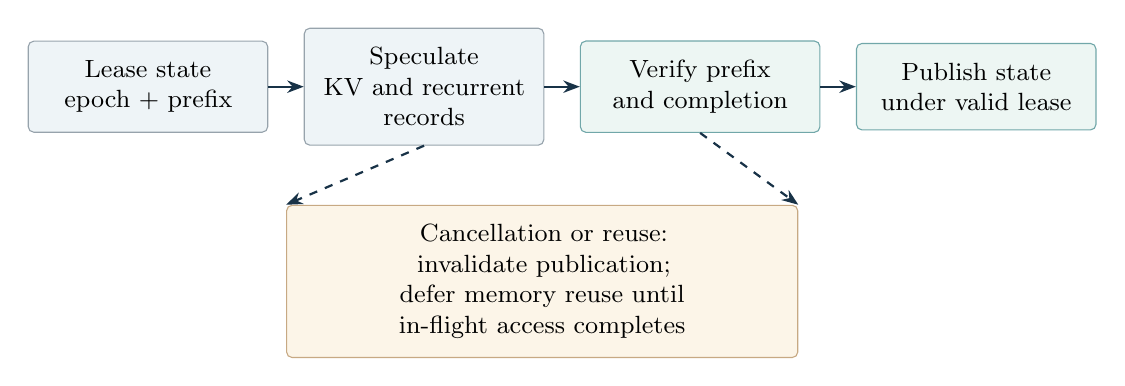
\begin{tikzpicture}[node distance=.45cm]
\node[box,text width=2.55cm] (lease) {Lease state\\epoch + prefix};
\node[box,text width=2.55cm,right=of lease] (spec) {Speculate\\KV and recurrent\\records};
\node[good,text width=2.55cm,right=of spec] (verify) {Verify prefix\\and completion};
\node[good,text width=2.55cm,right=of verify] (pub) {Publish state\\under valid lease};
\draw[flow] (lease)--(spec);\draw[flow] (spec)--(verify);\draw[flow] (verify)--(pub);
\node[warn,text width=6cm,below=.75cm of spec,xshift=1.5cm] (cancel) {Cancellation or reuse:\\invalidate publication;\\defer memory reuse until\\in-flight access completes};
\draw[dashedflow] (spec.south)--(cancel.north west);\draw[dashedflow] (verify.south)--(cancel.north east);
\end{tikzpicture}
\caption{State publication is a transaction. The included epoch model tests sequential publication guards; it does not prove CUDA memory ordering, race freedom or safe reclamation.}
\end{figure}

\subsection{Cache only what the continuation can legally reuse}
A prefix-state cache key must cover weights and adapters, positions, masks, relevant numerical/backend settings and every model-specific state component. SGLang's prefix-reuse work and FlashInfer's heterogeneous KV handling are existing substrates, not features invented here.\cite{sglangpaper,flashinfer} The proposed certificate cache adds its own namespace: the exact shared head, draft hidden vector or stable identifier, summary format, transform contract and position alignment.

Test shared-prefix divergence, eviction followed by recomputation, request reorder, cancelled requests, graph replay and slot recycling. Recurrent state cannot be reconstructed merely by finding matching attention pages. A retained head summary from a previous token is an alternate anchor only when its bound is recomputed for the new target hidden vector and all version conditions hold. The largest available cache is not necessarily best: evidence storage competes with KV capacity and can reduce admitted concurrency.

\section{A compiler interface for evidence and effects}\label{sec:compiler}
The compiler contribution should be small enough to implement and broad enough to explain the transformations. It need not replace the serving engine or invent a general-purpose language. Its input is an admitted tensor/state subgraph together with a consumer contract. Its output is a guarded implementation and an exact completion path.

\subsection{Decision types and legal rewrites}
An illustrative interface distinguishes values from demands:
\begin{lstlisting}
HeadSummary[head_version, row_alignment, score_contract]
Decision[TopK(k) | AcceptBit | ResidualSample | TargetSample | LogProbs]
StateLease[request_id, slot_epoch, materialized_prefix]
Evidence[enclosure_contract, covered_domain, producer_hash]

project_to_summary(W, hidden, consumer, evidence_layout)
transport(summary, delta, transform_contract) -> Evidence
refine(Evidence, demanded_tiles, numerical_backend) -> Evidence
resolve(Decision, Evidence, proposal_law, rng_key) -> result | unknown
commit(StateLease, verified_prefix, completion_metadata) -> published
\end{lstlisting}
These are proposed IR interfaces, not APIs already added to SGLang. Their purpose is to make illegal compositions visible. A top-$k$ summary cannot satisfy an unrestricted residual-sampling demand merely because it contains the proposed token. A state lease cannot be reused after cancellation. A real-arithmetic enclosure cannot discharge a bitwise comparison requirement without a numerical bridge.

Legal producer--consumer fusion requires more than matching shapes. The compiler checks extra consumers, observable aliases, intermediate casts, mutation, RNG effects and buffer lifetime. It may replace a materialized head with a top-$k$ epilogue when all consumers are satisfied. It may move a summary into that epilogue when doing so preserves the required logits and errors. It may not move normalization across a matrix product or drop a residual output used elsewhere. A search engine can explore legal implementations inside this boundary; its tensor equivalence result does not prove the stateful server around it.\cite{mirage}

\subsection{Evidence-producing transformations}
The structural search space contains four distinct operations. \emph{Elimination} removes unused outputs, such as a full logits tensor for an argmax consumer. \emph{Transport} reuses an earlier summary with a certified change bound. \emph{Refinement} replaces an uncertain summary with more precise computation. \emph{Publication} advances externally visible state only after the relevant decision is verified.

The first three form a useful algebra of partial knowledge. A refinement is ordered by the information it contains: every newly admitted interval must be a subset of the previous valid interval, or the old interval must be explicitly replaced by a separately valid bound without claiming monotonicity. A certificate is accepted only when all values consistent with the evidence produce the same demanded result. This design provides a checkable boundary between a proposing agent and the runtime.

A compact certificate ledger records the source and output hashes, head namespace, mathematical rule, numerical contract, covered shapes, unsupported cases and fallback. A separate runner tests the proposed artifact against an immutable reference. Candidate code may not inspect benchmark identities, read expected answers, edit the measurement harness or return cached outputs. The evidence path should be auditable without trusting the model that proposed the optimization.

\begin{figure}[t]
\centering
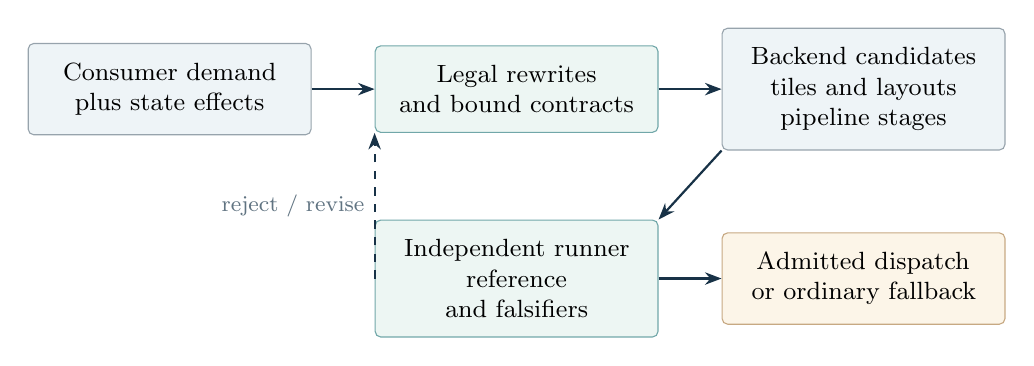
\begin{tikzpicture}[node distance=.8cm]
\node[box,text width=3.1cm] (demand) {Consumer demand\\plus state effects};
\node[good,text width=3.1cm,right=of demand] (rewrite) {Legal rewrites\\and bound contracts};
\node[box,text width=3.1cm,right=of rewrite] (backend) {Backend candidates\\tiles and layouts\\pipeline stages};
\node[good,text width=3.1cm,below=1.1cm of rewrite] (runner) {Independent runner\\reference and falsifiers};
\node[warn,text width=3.1cm,right=of runner] (admit) {Admitted dispatch\\or ordinary fallback};
\draw[flow] (demand)--(rewrite);\draw[flow] (rewrite)--(backend);
\draw[flow] (backend.south west)--(runner.north east);
\draw[flow] (runner)--(admit);
\draw[dashedflow] (runner.west)-|node[pos=.75,left,label]{reject / revise}(rewrite.south west);
\end{tikzpicture}
\caption{The proposed compiler boundary. Search may generate complicated implementations; admission remains tied to explicit semantics, numerical evidence and independent measurements. No end-to-end compiler has been implemented in this revision.}
\end{figure}

\subsection{The fusion portfolio remains broad}
The head is the main research mechanism, not a reason to ignore the rest of the trace. The full programme includes residual--normalization fusion, Q/K normalization with RoPE, gather--pack operations, accepted-prefix compaction, attention-backend dispatch, recurrent record layout, chunked prefill and removal of exposed synchronization. The requirement is that each intervention improve a measured dependency path and identify which baseline fusion already exists.

Draft-only quantization is an explicit arm: it can reduce proposal cost while retaining a fixed target under a correct actual-$q$ verifier. Target or KV quantization is another arm with a new numerical/quality baseline. Weight-only, FP8 and low-bit tensor-core formats should be compared only where the selected hardware and backend support them. A smaller representation can be slower at the actual batch size because dequantization, packing or occupancy dominates.

This broader portfolio also tests the central thesis. Some bottlenecks are best solved by a mature library kernel or a simpler scheduler, not a certificate. Keeping those alternatives in the experiment prevents a project about avoided work from spending more work defending its preferred mechanism than measuring it.

\section{Scheduling and structural autotuning}\label{sec:tuning}
\subsection{The scheduler chooses an execution regime}
An action includes verification depth, selector implementation, head strategy, refinement stage budget, backend, graph tier and state-flush policy. Its state includes request count, context lengths, deadlines, available KV capacity, recurrent-ring occupancy, certificate-mask geometry and the compiled implementations available. The intended optimization is useful committed progress under latency and memory constraints, not isolated kernel duration.

A restricted snapshot model remains valuable as an oracle. Let $F_i(d)$ be predicted progress for request $i$ at depth $d$ and suppose cost depends only on the total optional depth $m=\sum_i d_i$ at fixed state $z$. Then
\begin{equation}
G_i(m)=\max_{0\leq d\leq L_i}\{G_{i-1}(m-d)+F_i(d)\},\qquad
\max_m\frac{G_B(m)}{C(m;z)}\label{eq:schedDP}
\end{equation}
solves that snapshot by ordinary dynamic programming. The proof partitions allocations by the last request's depth, then enumerates totals. It is exact only under the cost hypothesis.

Real costs often violate it. Two allocations with the same total depth can use different context lengths, ring flushes or vocabulary-tile unions. One request may need a dense completion while another is certified immediately. The broader controller should price these effects rather than quietly calling~\eqref{eq:schedDP} optimal. A small exact exhaustive oracle on synthetic states can test a heuristic; it cannot prove online fairness or queue stability.

\subsection{Cliffs, unions and deadlines}
Graph tiers make cost discontinuous. With rewards $(1,1.9,2.7)$ and costs $(1,2,2)$ at depths $(0,1,2)$, depth one looks worse than zero while depth two is best. Stopping at the first local decline fails because the second token fills already-paid capacity. The test suite retains this witness.

A proposed richer cost approximation is
\begin{equation}
\widehat C(a;z)=C_{\rm backbone}(a;z)+C_{\rm state}(a;z)
+\sum_c b_c\ind\{c\in\cup_i A_i(a)\}/\widehat{\rm BW}
+C_{\rm row\mbox{-}tile}(a;z)+C_{\rm dispatch}(a;z).
\end{equation}
It separates shared weight bytes from active row--tile work. The fitted bandwidth and remaining terms must be validated on held-out shapes. A ring flush, an admission boundary or a backend switch can invalidate a smooth fit.

The online controller can use a short-horizon discrete action table or model-predictive search with a small action set. It should retain ordinary decoding, dense head evaluation and the upstream selector as admissible choices. Per-request deadlines and age limits bound any delay introduced by mask-affinity grouping. A throughput-only controller can otherwise repeatedly favour easy-to-certify requests and starve difficult ones.

For sampling, depth selection must obey Section~\ref{sec:stopping}. Head refinement order can depend on proposals because it preserves the fixed reference protocol. Altering proposal admission based on those same realized tokens requires a separate sampling argument. This distinction should be represented in the policy API, not left to reviewer intuition.

\subsection{Autotune structure before parameters}
The outer search changes what is computed: static screen, transported screen, retained-tail refinement, dense fusion, lazy selector, map selector, and their valid combinations. The inner search chooses implementation details: vocabulary and hidden tiles, row grouping, warps, stages, packing, epilogue layout, refinement batch size and the fallback threshold. Tuning the old shapes before changing the algorithm can optimize a regime the final system rarely executes.

Use a constrained objective over a frozen workload distribution,
\begin{equation}
\min_{a,\theta}\sum_{s\in\mathcal S_{\rm train}}w_sT(a,\theta;s)
\quad\text{subject to correctness, memory and regression constraints}.
\end{equation}
Retain a separate worst-case or tail-regression constraint. Begin with legal, diverse candidates and short paired measurements, then spend longer runs on survivors. Enumeration and successive screening are strong baselines for a small space; Bayesian or evolutionary search must justify its additional compilation and measurement budget. The proposing agent does not choose a new denominator after seeing results.

Autotuning a mutating kernel requires restoring all affected state, including RNG counters and ring occupancy, before each trial. Triton's autotuner explicitly provides reset/restore mechanisms because configurations execute more than once.\cite{tritonautotune} A candidate timed after another candidate changed its inputs has not been measured on the same problem. Compilation time, failed compilations and rejected resource layouts are part of the search evidence.

\subsection{Certificate selection as value of information}
Refinement scheduling introduces a further algorithmic question: which tile should be evaluated next? A large interval width is an easy reference heuristic, but a tile with a smaller interval may cross the actual acceptance threshold more cheaply. At batch scale, evaluating a shared tile can resolve several rows while paying its weight load once.

The programme should compare maximum-width refinement, threshold-distance heuristics, shared-tile gain estimates and a small oracle that knows the eventual logits. The oracle is an upper bound for replay analysis, never an online policy. A learned refinement policy can use only metadata available before the corresponding projection. Its objective is the reduction in expected remaining execution cost, including the possibility of dense completion. No optimality claim follows merely from calling the policy value-of-information.

\section{Experiments designed to decide the claim}\label{sec:experiments}
\subsection{Freeze the task and the baseline}
The first engine experiment is single-GPU, text-only and BF16, with a fixed model revision, reasoning mode, tokenizer, output limit, maximum context and server capacity. The head-sharing compatibility test is a precondition for the transport branch. The full programme then adds sampled decoding, mixed arrivals, longer contexts, a second model family and another hardware regime. These are cumulative tests of the claim, not substitutions for a failed primary baseline.

The required arms are optimized ordinary decoding, optimized existing speculation, and that same speculative configuration plus the contribution. The main speedup denominator is existing optimized speculation. Include the strongest compatible fused head/selection implementation, not merely eager \code{matmul + softmax}. Track the deployed backend with traces: a source file being present does not prove it was executed.

Launch each server arm once at its fixed maximum capacity and sweep client concurrency. Begin with $1,2,4,8,16,32$ where memory permits, declare a smaller supported ceiling when necessary, and add denser points around crossovers. Keep CUDA graphs and overlap features enabled in the production comparison. An instrumented run that forces synchronization is a diagnostic, not a performance baseline.

\subsection{Real-head replay before GPU specialization}
Collect aligned draft and target hidden inputs \emph{at the actual head boundary}, candidate IDs, proposal rows, target decisions, per-layer/state metadata, context lengths and the exact weight/configuration versions. Confirm position alignment with a few manually traceable cycles; the index predicting a token is not automatically the index consuming it.

On a prompt-disjoint held-out split, measure static and transported bounds, retained-tail tightening, certificate resolution, full-completion frequency, and masks' batch unions. Report distributions by position, domain, context length and acceptance outcome. Compare scalar, coordinate, grouped and low-rank residual geometries. Include unstructured or deliberately permuted tiles as controls, and measure any weight-repacking or metadata cost.

An offline evaluator may use dense target scores to determine the oracle answer, but the simulated online path may not use those scores until it pays for the corresponding row or tile. The supplied exact reference counts distinct requested rows through an explicit oracle object. Real replay tools must preserve this separation. Numerical double-precision replay is a useful bound-tightness screen, not a GPU rounding certificate.

\subsection{The ablation matrix}
\begin{table}[t]
\small\centering
\begin{tabularx}{\linewidth}{@{}P{.8cm}P{3.8cm}Y@{}}\toprule
Arm & Change from matched speculation & What it isolates \\\midrule
A0 & No change & Optimized speculative denominator.\\
A1 & Draft summary emission only & Cost of generating and retaining evidence.\\
A2 & Dense target head with fused consumer & Materialization and launch savings without skipped projection.\\
A3 & Static certified screen & Benefit obtainable without draft reuse.\\
A4 & Transported maxima & Greedy/top-$k$ certificate value.\\
A5 & Transported masses and acceptance guards & Decision value; exact residual/bonus retained.\\
A6 & A5 plus retained-tail refinement & Tightness versus seed-row cost.\\
A7 & A5 plus demand frontier & Avoided suffix head work under a fixed protocol.\\
A8 & Selected head path plus selector variants & Interaction with lattice, realized-row and map execution.\\
A9 & Selected paths plus state-aware scheduling & Incremental controller value and overhead.\\
A10 & Bounded residual and bonus races & Exact completion beyond the dense fallback, including priority-summary overhead.\\
A11 & Progressive precision certificates & Approximate computation used to preserve the fixed target.\\\bottomrule
\end{tabularx}
\caption{Ablations are implementation commitments for the research programme, not completed experiments. Any additional complement requires its isolated arm and a combined arm.}
\label{tab:ablations}
\end{table}
The four-way comparison baseline, $A$, $B$, $A+B$ is mandatory whenever two changes are composed. Do not multiply their isolated speedups. Summary generation can contend with draft selection; lazy projection can destroy batch weight reuse; state improvements can shift the best depth. Interactions are part of the result.

\subsection{Frontier metrics and useful throughput}
The requested frontier needs an explicit definition of tokens per second per user. For a reproducible end-to-end convention, let $n_i$ be the server-reported number of generated output tokens and $e_i$ the interval from request send to the last nonempty streamed output event. Define
\begin{equation}
x=\frac1N\sum_i\frac{n_i}{e_i},\qquad
y=\frac{\sum_i n_i}{t_{\rm last\ completion}-t_{\rm first\ send}}.
\label{eq:frontier}
\end{equation}
The $x$ axis is explicitly \emph{mean per-request end-to-end output rate}; it includes TTFT. For a decode-only frontier, also obtain a documented first-chunk token count and decode interval. Do not infer one token per SSE chunk or substitute the reciprocal of mean TPOT. AIPerf documents distinct latency and throughput measures and is a suitable primary benchmark client when pinned.\cite{aiperf}

Retain TTFT, end-to-end latency, inter-chunk timings, actual token counts, accept/progress histograms, head/commit time, graph hit rate, peak memory, error rate and completion reasons. If reasoning tokens are included in usage counts, keep that accounting consistent across arms. A fixed-length throughput panel should be separate from natural-stopping quality runs. Failures and timeouts remain in the report rather than being silently removed from a favourable mean.

Closed-loop concurrency sweeps locate the latency--throughput trade-off but do not establish open-loop service behaviour. Add fixed-arrival-rate tests near the operating knee, mixed prefill/decode traffic and bursts. Report offered load, completed requests, failures and SLO-constrained useful throughput. Test cold prefixes and explicitly declared shared-prefix workloads separately. The same repeated prompt is not an unbiased proxy for arbitrary traffic.

\subsection{Quality, reliability and statistical power}
For a purportedly exact greedy change, compare complete continuations against the admitted reference and record every mismatch. A task benchmark alone cannot validate numerical equality. For sampling, use exact finite-distribution tests, coupled decision tests and real-model distribution/quality checks appropriate to the admitted contract. Identical sampled text under one seed is neither necessary nor sufficient for equality in distribution.

Use text, code, mathematics, structured output and multilingual prompts where the selected model supports them. Baseline quality before target quantization or post-training, with a fixed task set and prompt split. Report the model change's quality/performance trade-off separately from exact execution changes. For draft-only approximation, report actual proposal support, acceptance and cycle cost even when target quality is preserved by construction.

Use exploratory runs to choose candidates, then freeze them. At key low-latency points and the throughput knee, perform at least five paired runs with alternating order on an otherwise idle GPU; increase repetitions for close effects. Resample paired runs and prompt clusters, not individual tokens as though they were independent. Report confidence intervals, all tested concurrency points and regressions. A sparse sample cannot support a persuasive p99. Selection on the best-looking point of the same noisy sweep is not a confirmatory result.

\subsection{Failure criteria are part of the programme}
\begin{longtable}{@{}P{3.3cm}P{5.0cm}P{6.0cm}@{}}
\toprule Hypothesis & Fastest damaging test & Response if it fails \\\midrule\endhead
Transport is tighter than a static screen & Aligned real-head replay, including high-entropy and off-domain contexts & Improve head-metric geometry or use a different anchor; retain dense/fused execution.\\
Certificates save target work & Count rows, tiles and complete residual/bonus work, not just decision cost & Reject an acceptance-only speed claim; investigate exact completion separately.\\
Sparsity saves weight bandwidth & Measure union masks and real HBM/L2 traffic & Group compatible rows, use coarse masks or switch to dense GEMM.\\
Fusion preserves the target & Close-logit, tie and cast-point tests with admitted numerical reference & Restore rounding, enclose reference error, or disclose a different contract.\\
The controller is cheap & Concurrency-one and graph-tier crossover measurements & Use static dispatch in that region; do not amortize imaginary overhead.\\
More lookahead improves acceptance & Fixed-anchor replay against greedy and an oracle coverage ceiling & Improve the predictor or retain the greedy selector; optimizer sophistication is not evidence.\\
State replay is equivalent & Every rejection position, ring boundary and cache-restoration path & Correct the state model before timing; inspect raw versus derived records.\\
Adaptive sampling remains exact & Exhaustive tiny laws including candidate-dependent stopping & Restrict policy information or derive the actual joint correction law.\\
Transfer is real & New prompts, context distributions, model/head geometry and GPU regime & Narrow the supported claim and explain the dependency.\\\bottomrule
\end{longtable}
The response to a failed hypothesis is not to erase it from the paper. A negative result that rules out an attractive but wrong systems argument is useful evidence. The programme stays ambitious by testing stronger alternatives, not by weakening the meaning of correctness or changing the comparison after the fact.

\section{Evidence produced in this revision}\label{sec:evidence}
\subsection{Exact references and executed tests}
The new decision reference uses bounded integer head weights and hidden vectors. A logit $z$ has unnormalized mass $2^z$, represented exactly with rational arithmetic; this is equivalent to an exponential model with logits scaled by $\log 2$. It avoids trusting floating exponentials while exercising the same certificate and rejection identities. It is not an evaluation of a trained model.

Eighteen new test methods in the decision reference and three in the race reference passed. Four additional tests exercised the local benchmark-client protocol. Table~\ref{tab:tests} reports generated finite instances inside them. Counts are not independent confirmations of an LLM deployment. The seed, environment versions, commands and JSON results are in the bundle. The test harness uses a target-row oracle that projects only requested rows, so work counts do not silently evaluate the full target first.

\begin{table}[t]
\small\centering
\begin{tabularx}{\linewidth}{@{}P{5cm}rY@{}}\toprule
Check & Executed count & Scope \\\midrule
Top-$k$ plus tail composition & 250 & Exact union and associative merge.\\
Transported tile bounds & 300 heads; 1,048 tiles & 3,787 weight rows enclosed.\\
Greedy certified screening & 250 & Same winner under a deterministic total order.\\
Retained-tail tightening & 565 tiles & Exact mass enclosed; bounds no looser.\\
Acceptance interval guards & 1,600 & Certified bits agree with complete mass.\\
Unresolved interval measure & 160 & Exact agreement with Equation~\eqref{eq:unknown}.\\
Lazy acceptance & 500 & With/without retained seeds; finite completion.\\
Coupled one-step sampling & 200 & Same output with exact residual fallback.\\
Rejection-correction identity & 300 pairs & Includes zero-probability support entries.\\
Demand frontier & 1,092 partial states & 5,460 complete decision assignments.\\
Exclusion-aware race summaries & 300 & Exact maxima after support exclusions.\\
Target priority race & 250 & Same token as a dense priority race.\\
Sparse-support residual race & 250 & Exact bounded/dense race equivalence.\\
Finite-map execution & 400 & Scan/walk and composition agreement.\\
Gated-delta replay & 150 trajectories & 868 accepted-prefix replay checks.\\
Lease reuse & 300 schedules & Sequential epoch and base-prefix guards.\\\bottomrule
\end{tabularx}
\caption{New CPU evidence. Additional explicit counterexamples cover biased depth selection, graph-cost cliffs, batch unions, invalid numerical bounds, support truncation and stale namespaces. No GPU implementation is exercised.}
\label{tab:tests}
\end{table}
The earlier v2 suite was rerun separately, retaining its nine test methods. The v1 exhaustive prefix/certificate suite was also rerun. Their sources and logs remain separately named, rather than being merged into a larger number that suggests independent implementations of the same claim. Neither inherited suite establishes real-model certificate tightness.

\subsection{A synthetic experiment that exposes the wrong denominator}
The drift experiment constructs two families of $128\times8$ integer heads, with vocabulary tiles of 16 rows and 36 paired fixtures per family. One family deliberately clusters weight rows around separated centres; the control uses unstructured rows. For each fixture, $h^t=h^d+d\,v$ with integer drift scale $d\in\{0,1,2,4\}$. Proposals are sampled from the \emph{anchor-head} categorical law, not from a trained DFlash2 selector. All probability arithmetic is exact.

At zero drift, the summaries describe the target exactly, so the acceptance decision needs only its candidate row. This $1/128$ row fraction is an identity sanity check, not a realistic speed forecast. At nonzero drift, the unstructured head largely defeats greedy screening. More subtly, large drift can make rejection easy to certify, reducing the acceptance-test work while destroying acceptance itself. Completing the residual then erases almost all of that apparent saving.

\begin{table}[t]
\small\centering
\begin{tabular}{@{}lrrrrr@{}}\toprule
Head family & Drift & Greedy rows & Decision rows & Decision + residual & Accepted \\\midrule
Clustered & 0 & 13.2\% & 0.8\% & 0.8\% & 100.0\%\\
Clustered & 1 & 40.3\% & 21.9\% & 76.8\% & 36.1\%\\
Clustered & 4 & 51.3\% & 11.4\% & 96.5\% & 5.6\%\\
Unstructured & 0 & 13.9\% & 0.8\% & 0.8\% & 100.0\%\\
Unstructured & 1 & 99.7\% & 64.0\% & 98.6\% & 50.0\%\\
Unstructured & 4 & 100.0\% & 22.4\% & 100.0\% & 5.6\%\\\bottomrule
\end{tabular}
\caption{Executed synthetic work counts, not timings. Row fractions count distinct target rows projected. ``Decision + residual'' completes all target rows on rejection. It still excludes draft evidence production, bounds, bonus sampling and the target backbone. Full data, including drift two and retained-tail variants, are in the CSV.}
\label{tab:drift}
\end{table}
At drift four, the clustered family's decision-only row fraction is $11.4\%$, but including exact residual completion raises it to $96.5\%$. In the unstructured family it reaches $100\%$. This is why an acceptance-kernel benchmark by itself would be an inadequate result. The experiment does not refute transported certificates on trained heads; it refutes the inference that a cheap acceptance decision necessarily means cheap verification.

\subsection{Formal evidence status}
The manuscript contains complete mathematical proofs of the stated certificate and structural implications. A small Lean source file provides nine proof declarations for scaled-integer guards, refinement monotonicity, function composition, deterministic replay and lease publication. It contains no placeholder proofs or added axioms, but it was \emph{not compiled}: no Lean executable was available in the authoring environment and attempts to obtain one were unsuccessful. The build script fails explicitly when validation is unavailable.

These sources are therefore a formalization draft, not machine-checked evidence. Even successful compilation would not prove floating-point head enclosures, the rational representation bridge, CUDA memory ordering, a trained proposal law or the complete compiler. Those remaining obligations are listed beside the proof source. A small verified decision checker is useful; claiming that it verifies the server would not be.

\subsection{What is still unknown}
There is no trained-model hidden-state trace, checkpoint-specific bound calibration, compiled GPU fast path, sanitizer run, on-policy serving result or quality evaluation in this revision. In particular, we do not know whether the head-metric residuals are small enough, whether useful sparse masks share tiles across requests, or whether the additional draft epilogue is affordable. Those are the next experiments, not qualifications to be removed once the paper is formatted.

\section{What the completed paper should establish}\label{sec:conclusion}
The full research programme asks whether speculative execution can be compiled around the evidence a verifier needs, rather than around the tensors an existing implementation happens to materialize. The shared-head path gives this question a concrete mathematical and engineering form. A drafter's projection becomes evidence; target work refines that evidence only where a decision remains unresolved; state publication preserves the verified prefix.

The programme is deliberately broader than one kernel. It includes alternate selector execution, head-metric learning, progressive-precision certificates, state transactions, graph-aware scheduling and structural autotuning. Their purpose is not to accumulate impressive-sounding components. It is to find which forms of avoided work survive the constraints that usually undo them: uncertainty, numerical rounding, lost parallelism, shared memory traffic and completion costs.

A successful paper would show a repeatable improvement in the optimized server's frontier, isolate the mechanism, and explain where it stops working. A useful negative paper would establish that a tempting source of reuse cannot pay for itself on realistic geometry or batching, with a clear account of why. The present artifact supplies the mathematical boundaries, executable falsifiers and implementation contracts needed to tell those outcomes apart.

\appendix
\section{Integration contracts and source seams}\label{app:integration}
The primary engine audit uses SGLang commit
\begin{center}\small\texttt{bd66ce343e4f6e2f2b75d7e820fe4d0718a8d824}.\end{center}
This is a frozen research pin, not a claim that its checkout is the latest revision or the correct production deployment. Model revisions and the selected runtime backend must be recorded during implementation.

\begin{longtable}{@{}P{4.7cm}P{9.6cm}@{}}\toprule
Path under \code{python/sglang/} & Proposed integration and invariant \\\midrule\endhead
\path{srt/models/dflash.py} & Extend the actual shared-head candidate producer with evidence output. Preserve dense/quantized distinctions, original vocabulary bounds and the reference candidate ordering. Read \code{candidate\_topk} and its producer rather than adding a second gratuitous head pass.\\
\path{srt/layers/logits_processor.py} & Admit a decision-specific target-head consumer only when every output consumer is satisfied. Arbitrary log-probabilities and unsupported transforms retain the ordinary path. This is a proposed seam, not an implemented patch.\\
\path{srt/speculative/dflash_worker_v2.py} & Carry aligned evidence, actual proposal law, masks and completion metadata through stable graph buffers. Preserve the captured tail and request identity. Audit the exact worker revision before editing.\\
\path{kernels/ops/speculative/dflash.py} & Compare existing walk, realized-row score/walk, and map-producing score implementations. Maintain RNG and arithmetic contracts.\\
\path{srt/layers/attention/linear/gdn_backend.py} & Identify which recurrent backend is actually selected. Integrate only after tracking its consumed-token indexing and state layout.\\
\path{kernels/ops/attention/fla/gdn_replayssm_spec_fold.py} & Existing raw-input fold with explicit numerical-order restrictions. Its \code{accept\_lens} comment includes a bonus in that backend's indexing; map this convention to emitted and materialized prefixes rather than assuming a universal length formula.\\\bottomrule
\end{longtable}
Only the existing code observations are source claims. The new producer, demand types, evidence buffers and controller described here remain proposed engineering work. A file-level audit does not demonstrate runtime dispatch or GPU correctness.

\subsection{Proposed evidence ABI}
For $B$ requests, $L$ proposed positions and $C$ vocabulary tiles, store row alignment and epoch identifiers, anchor hidden vectors when required, tile maxima and log-mass enclosures, optional retained IDs and tail summaries, and the head/transform namespace. Separate immutable checkpoint geometry from per-cycle evidence. Use structure-of-arrays layouts for fields consumed together by bound and decision kernels.

A reasonable first layout has FP32 maxima, log-mass bounds and centre shifts; 32-bit token IDs and tile masks; and 64-bit epochs where wraparound would otherwise require a protocol. These are design choices to validate, not a proof that FP32 is sufficient for certification. Interval formats must represent outward bounds or use a tested error inflation. Fixed buffers require explicit valid lengths for vocabulary tails, padded positions and cancelled requests.

The epoch identity is not a floating tensor annotation that can be dropped by compilation. It is part of the publication protocol. The dispatcher may use an opaque version handle rather than hash the entire weight matrix per cycle, but the handle must be invalidated when weights, adapters, relevant packing or transforms change.

\subsection{A fixed-stage GPU sketch}
\begin{lstlisting}
# Proposed execution, not an existing kernel implementation.
# Input proposal block and RNG assignment are fixed by the reference protocol.
summary = draft_head_with_evidence(draft_hidden, shared_W)
target_hidden, private_state = target_verify_backbone(proposals)
evidence = transport(summary, target_hidden - draft_hidden)
seeds = target_candidate_scores(target_hidden, proposals)
status = resolve_guards(evidence, seeds, actual_q, reference_uniforms)

for stage in STATIC_REFINEMENT_STAGES:
    frontier = first_certified_rejection(status)
    work = choose_tiles(evidence, unresolved_before(frontier), graph_budget)
    exact_tiles = project_selected_tiles(target_hidden, shared_W, work)
    evidence = refine_with_valid_bounds(evidence, exact_tiles)
    status = resolve_guards(evidence, seeds, actual_q, reference_uniforms)

complete_unresolved_reference_rows()
sample_exact_residual_or_bonus()
restore_and_publish_verified_state(current_lease)
\end{lstlisting}
Every stage is bounded and uses stable buffers. A real graph implementation must handle mixed request states without host synchronization, respect legal kernel boundaries and preserve the lifetime of private speculative state. ``Choose tiles'' may be approximate as a cost policy because fallback preserves correctness; ``valid bounds'' may not be approximate as a soundness policy.

\section{Mathematical extensions and additional falsifiers}\label{app:math}
\subsection{An evidence envelope for transformed logits}
Suppose a target transform changes logits by a known per-token correction $b_i$, and a tile has valid bounds $b_c^-\leq b_i\leq b_c^+$. Adding these to~\eqref{eq:transport-row} gives
\begin{equation}
z_i^d+a_c-\epsilon_c+b_c^-\leq z_i^t+b_i
\leq z_i^d+a_c+\epsilon_c+b_c^+.
\end{equation}
The corresponding mass bounds multiply by $e^{b_c^-}$ and $e^{b_c^+}$. This is useful only when the bounds refer to the actual transformed domain. A mask that deletes unknown members cannot preserve the unmasked lower mass; a safe lower bound may collapse to zero. Positive temperature scaling can be incorporated by scaling logits and bounds consistently, but using an old mass at a new temperature generally requires more than multiplying the old mass by a scalar.

\subsection{Why one anchor mass is insufficient under arbitrary temperature change}
Two tiles can have equal $\sum_i e^{z_i}$ and different $\sum_i e^{\lambda z_i}$ for $\lambda\neq1$. For example, the unnormalized masses $(1,3)$ and $(2,2)$ both sum to four, while their squares sum to ten and eight. A changed-temperature mass cannot be reconstructed from the old sum alone. Retained scores, additional moment summaries or conservative bounds can help, but they add cost. This prevents a seemingly harmless extension from silently using the wrong normalizer.

\subsection{A conditional rate certificate}
If valid positive intervals enclose candidate and baseline expected progress and time, a sufficient rate-improvement certificate is
\begin{equation}
\frac{R_1^-}{T_1^+}>\frac{R_0^+}{T_0^-}.
\end{equation}
The proof is monotonicity of division by a positive denominator. These intervals are assumptions. A small benchmark confidence interval, a fitted cost table and an average calibration score do not automatically form simultaneous deterministic enclosures. Use this inequality to expose what must be estimated, not to market a certified production speedup.

\subsection{A lower limit on what summaries can establish}
Without an error envelope, agreement at an anchor gives no guarantee away from it. Let $h^d=(1,0)$ and $h^t=(1,1)$. Weight rows with the same first coordinate have identical anchor logits, while their second coordinates can make the target logits arbitrarily different. An anchor maximum or mass alone cannot certify the target. A geometric residual bound, additional projection information, or exact completion is necessary. This elementary construction is why the shared-head idea needs a certificate rather than a similarity heuristic.

\subsection{Sampling-policy and RNG tests}
Preserve a counter-based mapping from request, cycle, position and draw purpose to reference randomness, or explicitly disclose that only distributional rather than seeded equality is intended. Extra Gumbel draws for unused predecessor rows must not accidentally advance a shared generator and change later requests. A map-based sampled selector needs the realized proposal row after the path is known, not merely its selected ID.

Exhaustive tiny-law tests should cover point-mass proposals, zero support, $p=q$, acceptance at the comparison boundary, all-accept cycles, first-position rejection and candidate-dependent stopping. Coupled tests should keep proposal draws, acceptance uniforms and residual uniforms aligned. The reference suite covers one-step coupling and frontier decisions, not a complete trained autoregressive sequence or the engine's RNG implementation.

\section{The implementation programme is cumulative}\label{app:programme}
The work is organized by evidence dependencies, not by a promise that the entire research programme fits the take-home's initial allocation. The first executable slice should be small enough to measure; the research scope is larger and remains intact.

\begin{longtable}{@{}P{1.2cm}P{5.1cm}P{8.0cm}@{}}\toprule
Stage & Deliverable & Evidence required to advance \\\midrule\endhead
I & Frozen optimized engine and workload; head/state critical-path traces & Runtime backend identified; graph and overlap confirmed; ordinary and existing speculative frontiers saved.\\
II & Aligned real-head replay and bound geometry & Correct row alignment; prompt-disjoint data; numerator, mass, tile-union and completion-cost distributions.\\
III & Dense fused head plus evidence epilogue & Candidate/probability contract tests; isolated evidence overhead; strong dense comparator.\\
IV & Greedy transported screen and progressive refinement & Numerical enclosure admission; tie tests; fallback; real saved traffic; before/after serving curve.\\
V & Sampled acceptance certificates and exact completion & Actual-$q$ law, RNG coupling, residual/bonus correctness, candidate-dependent stopping exclusions.\\
VI & Selector execution portfolio and prefix-value study & Exact paths for structural variants; held-out acceptance for learned objectives; joint head interaction ablations.\\
VII & Hybrid-state transactions and joint dispatch & All rejection positions, flush boundaries, cancellation and reuse tests; race/memory checks; tail-latency guardrails.\\
VIII & Head-metric training, progressive precision and transfer & Training cost and quality controls; admitted precision envelopes; second model/GPU and held-out workload.\\\bottomrule
\end{longtable}
The stages permit parallel research where dependencies allow it. A geometry investigation can proceed alongside a state audit and compiler design. GPU time should be spent on hardware questions, while exact references, proof work and data analysis can run on CPU. Every branch retains its failed candidates and records the reason for rejection.

The first presentation can lead with one defensible result and show how it opens the broader programme. It should not present unimplemented stages as accomplishments. The full paper earns its scope by connecting each result to the central claim and identifying which assumptions the next stage tests.

\section{Artifact, reproduction and remaining proof work}\label{app:artifact}
The bundle contains a standalone manuscript source, compiled PDF, exact CPU references, the inherited reference suites, tests, a synthetic work-count experiment, JSON/CSV evidence, a small benchmark client, a proposed experiment contract, a source manifest and the formalization draft. No confidential assignment or downloaded model weights are redistributed.

Run the CPU evidence from the bundle root:
\begin{lstlisting}
python tests/test_decisions.py
python tests/test_races.py
python tests/test_benchmark_client.py
python tests/test_v2.py
python src/v1_reference.py --output evidence/v1_tests.json
python experiments/synthetic_drift.py
bash scripts/check_lean.sh   # fails if Lean is unavailable
\end{lstlisting}
All Python commands above were executed during preparation. The Lean check did not compile a theorem file. The supplied toolchain pin is a build target, not a claim of successful validation. Future proof work should first compile these small guard lemmas, then formalize finite-domain mass transport and the bridge from rational comparisons to the admitted numerical implementation. Proving only an abstract inequality leaves the most important GPU assumption outside the checker.

The benchmark client provides raw request records and explicit accounting. Its local protocol smoke test is not an engine benchmark. Real server runs require the user's selected GPU, loaded checkpoint and frozen configuration. AIPerf remains the primary comparison client where its supported metrics and dataset features match the experiment. The source manifest records inspected publications and code seams; it does not invent unavailable model commit hashes.

\subsection*{Attribution and disclosure}
This manuscript, derivations and reference code were prepared with GPT-6 Astra Pro (OpenAI), using the supplied research materials, public primary sources and local CPU execution. Samuel Mausberg is the intended author and should review the claims and implementation before external submission. No independent human review, real-model evaluation, GPU validation or machine-checked Lean compilation is asserted. The confidential assignment is not included, and public release remains subject to the applicable sharing permissions.

\begin{thebibliography}{40}
\small
\bibitem{sgcode} SGLang contributors. \emph{DFlash model and candidate-head implementation}. Frozen commit \sourcepin, \path{python/sglang/srt/models/dflash.py}. \url{https://github.com/sgl-project/sglang/blob/bd66ce343e4f6e2f2b75d7e820fe4d0718a8d824/python/sglang/srt/models/dflash.py}.
\bibitem{qwenconfig} Qwen. \emph{Qwen3.5-4B configuration}. Inspected 30 September 2026; deployment revision still to be pinned. \url{https://huggingface.co/Qwen/Qwen3.5-4B/raw/main/config.json}.
\bibitem{qwencard} Qwen. \emph{Qwen3.5-4B model card}. \url{https://huggingface.co/Qwen/Qwen3.5-4B}.
\bibitem{dflashcard} Inco AI. \emph{Qwen3.8-27B-DFlash2 model card}. \url{https://huggingface.co/incoai/Qwen3.8-27B-DFlash2}.
\bibitem{dflash} Inco AI. \emph{DFlash 2: Keep Drafting Parallel}. 18 August 2026. \url{https://inco.ai/blog/dflash2/}.
\bibitem{flashsampling} Tomas Ruiz et al. \emph{FlashSampling: Fast and Memory-Efficient Exact Sampling}. arXiv:2603.15854v2, 12 May 2026. \url{https://arxiv.org/html/2603.15854v2}.
\bibitem{sonic} \emph{SonicSampler: Unified Tile-Aware Kernels for LLM Sampling and Speculative Verification}. arXiv:2607.20475v1. \url{https://arxiv.org/html/2607.20475v1}.
\bibitem{specvocab} Williams et al. \emph{Speculative Decoding with a Speculative Vocabulary}. arXiv:2602.13836v2, 17 July 2026. \url{https://arxiv.org/html/2602.13836v2}.
\bibitem{dynaspec} \emph{DynaSpec: Context-aware Dynamic Speculative Sampling for Large-Vocabulary Language Models}. Versioned manuscript, arXiv:2510.13847v3, 3 February 2026. \url{https://arxiv.org/html/2510.13847v3}.
\bibitem{microspec} \emph{MicroSpec: Accelerating Speculative Decoding with Lightweight In-Context Vocabularies}. arXiv:2605.26444v1. The unversioned abstract surfaced a different title during this audit; this citation refers specifically to v1. \url{https://arxiv.org/html/2605.26444v1}.
\bibitem{replayssm} Dao AI Lab. \emph{ReplaySSM: Cache SSM Inputs, Not State}. 2026. \url{https://dao-lab.ai/blog/2026/replayssm/}.
\bibitem{gdncode} SGLang contributors. \emph{GDN ReplaySSM speculative fold}. Frozen commit \sourcepin. \url{https://github.com/sgl-project/sglang/blob/bd66ce343e4f6e2f2b75d7e820fe4d0718a8d824/python/sglang/kernels/ops/attention/fla/gdn_replayssm_spec_fold.py}.
\bibitem{opttree} \emph{OPT-Tree: Speculative Decoding with Adaptive Draft Tree Structure}. arXiv:2406.17276. \url{https://arxiv.org/abs/2406.17276}.
\bibitem{dcut} \emph{D-cut: Adaptive Verification Depth Pruning for Batched Speculative Decoding}. arXiv:2607.14647. \url{https://arxiv.org/abs/2607.14647}.
\bibitem{pr36136} SGLang PR 36136. \emph{Dynamic verification for DFlash2}. Inspected open/unmerged, 30 September 2026; head \texttt{c0235e700214f1de5044be25f795faf5b755e450}. \url{https://github.com/sgl-project/sglang/pull/36136}.
\bibitem{mirage} Mengdi Wu et al. \emph{Mirage: A Multi-Level Superoptimizer for Tensor Programs}. OSDI 2025; arXiv:2405.05751v3. \url{https://arxiv.org/abs/2405.05751}.
\bibitem{lilicorr} Rusanovsky et al. \emph{LiLiCorr: Lightweight Likelihood Correlation of Parallel Drafts for Speculative Decoding}. arXiv:2608.20530v2, 22 September 2026. \url{https://arxiv.org/html/2608.20530v2}.
\bibitem{astar} Chris J. Maddison, Daniel Tarlow and Tom Minka. \emph{A* Sampling}. 2014. \url{https://arxiv.org/abs/1411.0030}.
\bibitem{specdecode} Yaniv Leviathan, Matan Kalman and Yossi Matias. \emph{Fast Inference from Transformers via Speculative Decoding}. ICML 2023; arXiv:2211.17192. \url{https://arxiv.org/abs/2211.17192}.
\bibitem{floatguide} NVIDIA. \emph{Floating Point and IEEE 754}. Documentation inspected 30 September 2026. \url{https://docs.nvidia.com/cuda/floating-point/index.html}.
\bibitem{torchnumeric} PyTorch. \emph{Numerical accuracy}. \url{https://docs.pytorch.org/docs/stable/notes/numerical_accuracy.html}.
\bibitem{torchtopk} PyTorch. \emph{torch.topk}. Tie-stability qualification. \url{https://docs.pytorch.org/docs/stable/generated/torch.topk.html}.
\bibitem{flashinferapi} FlashInfer. \emph{Sampling API}. Documentation inspected 30 September 2026. \url{https://docs.flashinfer.ai/api/sampling.html}.
\bibitem{cute} NVIDIA CUTLASS. \emph{CuTe DSL overview}. \url{https://docs.nvidia.com/cutlass/latest/media/docs/pythonDSL/overview.html}.
\bibitem{tilelang} TileLang contributors. \emph{TileLang documentation}. \url{https://tilelang.com/}.
\bibitem{tritonautotune} Triton contributors. \emph{triton.autotune}. Configuration pruning and reset/restore semantics. \url{https://triton-lang.org/main/python-api/generated/triton.autotune.html}.
\bibitem{hopper} NVIDIA. \emph{Hopper Tuning Guide}. CUDA 13.0.2 archive. \url{https://docs.nvidia.com/cuda/archive/13.0.2/hopper-tuning-guide/index.html}.
\bibitem{blackwell} NVIDIA. \emph{Blackwell Tuning Guide}. CUDA 13.4 documentation inspected 30 September 2026. \url{https://docs.nvidia.com/cuda/blackwell-tuning-guide/index.html}.
\bibitem{vllmgraphs} vLLM contributors. \emph{CUDA Graphs design}. \url{https://docs.vllm.ai/en/latest/design/cuda_graphs/}.
\bibitem{nsight} NVIDIA. \emph{Nsight Compute Profiling Guide}. \url{https://docs.nvidia.com/nsight-compute/ProfilingGuide/index.html}.
\bibitem{gdn} Songlin Yang, Jan Kautz and Ali Hatamizadeh. \emph{Gated Delta Networks: Improving Mamba2 with Delta Rule}. ICLR 2025; arXiv:2412.06464v3. \url{https://arxiv.org/abs/2412.06464}.
\bibitem{sglangpaper} Lianmin Zheng et al. \emph{SGLang: Efficient Execution of Structured Language Model Programs}. arXiv:2312.07104v2. \url{https://arxiv.org/abs/2312.07104}.
\bibitem{flashinfer} Zihao Ye et al. \emph{FlashInfer: Efficient and Customizable Attention Engine for LLM Inference Serving}. MLSys 2025; arXiv:2501.01005v2. \url{https://arxiv.org/abs/2501.01005}.
\bibitem{aiperf} NVIDIA. \emph{AIPerf Metrics Reference}. \url{https://docs.nvidia.com/aiperf/reference/ai-perf-metrics-reference}.
\end{thebibliography}
\end{document}
